\chapter{Resultados}
\label{chap:resultados}

Em vista dos procedimentos teóricos aliados a uma solução computacional, obteve-se resultados sequênciais de processamento de áudio. Tais resultados são:
\begin{itemize}
    \item resultado da resposta em frequência;
    \item resultado da sugestão de notas;
    \item resultado da sugestão de acordes;
    \item resultado da detecção de transições rítmicas;
    \item resultado da implementação da transformada wavelets;
    \item resultado da transcrição de notas;
    \item resultado da tonalidade do áudio;
    \item resultado da transcrição automática de acordes ao longo do tempo.
\end{itemize}

A primeira camada (Anexo 1, A3) de processamento da solução computacional proposta é a relativa a transformada de fourier. O resultado dessa camada é um vetor de 22.050 posições. Cada posição referente a frequência e sua resposta o valor da mesma.

A segunda camada (Anexo 1, A5) é a da rede neural para sugestão de notas. Ela tem como insumo de entrada a transformada de fourier. O resultado dessa camada é um vetor de 12 posições. Cada posição é representada por uma nota musical.

A terceira camada (Anexo 1, A6) é a da rede neural para sugestão de acordes. Ela tem como insumo de entrada as sugestões de notas da rede neural anterior. O resultado dessa camada é um vetor de 48 posições. Cada posição é representada por um tipo de acorde diferente entre as possibilidades de acorde maior, menor, aumento e diminuto para cada nota musical.

Para a demonstração de tais resultados foram feitos experimentos com todas as possibilidades de detecção de acordes proporcionados pelo sistema. Todavia serão detalhados e comentados somente 4 pois para os outros equivalem as mesmas considerações. O resumo dos resultados dos outros experimentos estará presente na tabela que se segue logo após. Esses experimentos foram feitos levando em consideração pré-condições e pós-condições.
\newpage

\section{Pré-condições dos Experimentos}
\label{sec:precondicoes}

No que tange às pré-condições foram levados em conta:
\begin{itemize}
    \item teclado yamaha E413 com som de piano para a execução dos acordes;
    \item somente tríades (3 notas) tocadas;
    \item o software Audacity \footnote{http://www.audacity.sourceforge.net} foi utilizado para gravação;
    \item o microfone convencional interno do $notebook$ foi utilizado para aquisição dos sinais de áudio;
    \item o ruído de fundo estava com uma grandeza por volta de 45 db;
    \item a taxa de amostragem do sinal foi configurada em 44100 Hz;
    \item gravação do áudio no formato de arquivo .wav em codificação 16 pcm.
    \item inicialização do software Scilab;
    \item execução do comando para importar a função principal do sistema (Anexo, A1): exec dc.sci;
    \item abertura do arquivo de áudio: audio = wavread('arquivo.wav');
    \item execução do algorítmo tendo o áudio gravado como parâmetro: acorde = DA2(audio);
    \item o resultado do acorde tocado estará guardado na variável acorde;
    \item para a geração de resultados automáticos com todas as amostras representantes de todas as possibilidades de acordes, faz-se necessário da execução do seguinte comando (Anexo, A11): exec acordes{\_}test.sci.
\end{itemize}

\newpage
As tríades de acordes foram executadas com base na nota central $C4$ que possui o valor de aproximadamente 261,6 Hz. Segue uma foto ilustrativa das regiões e limites usados \cite{teclado}:

\begin{figure}[h]
	\centering
		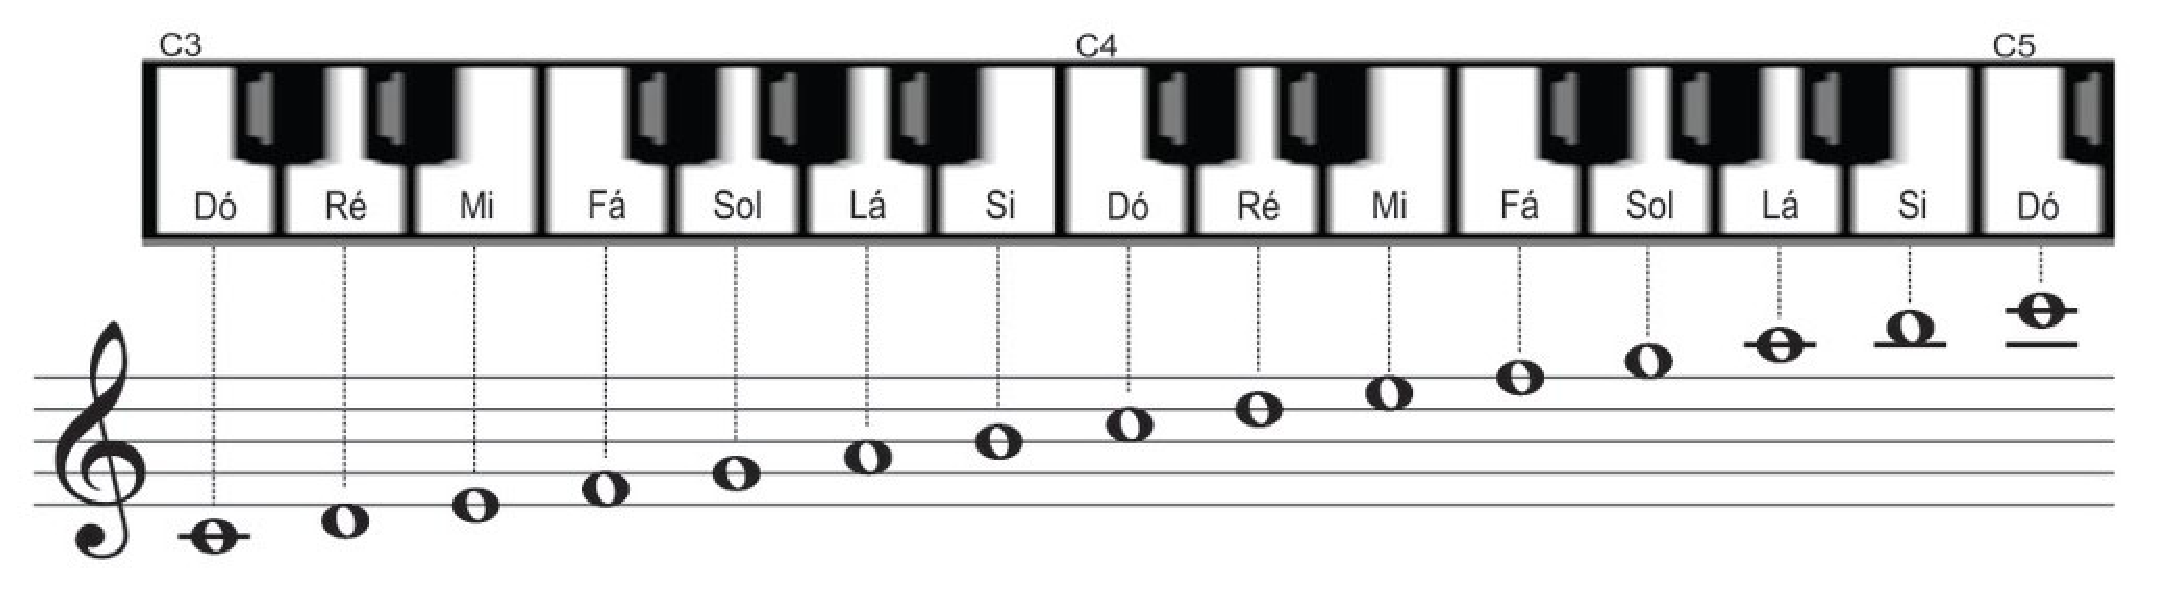
\includegraphics[keepaspectratio=true,scale=0.4]{figuras/teclado-tcc1.eps}
	\caption{Teclado ilustrativo para execução dos acordes}
\end{figure}

O processo de execução do experimento foi dividido em 4 etapas. A primeira relativa a gravação do acorde tocado no teclado via microfone convencional interno do $notebook$. A segunda é a exportação do som no formato de arquivo .wav pelo software audacity. A terceira etapa é a introdução do arquivo na entrada do sistema de detecção de acordes. A última atividade é a classificação do arquivo digital num acorde. Segue esquema ilustrativo do processo:

\begin{figure}[h]
	\centering
		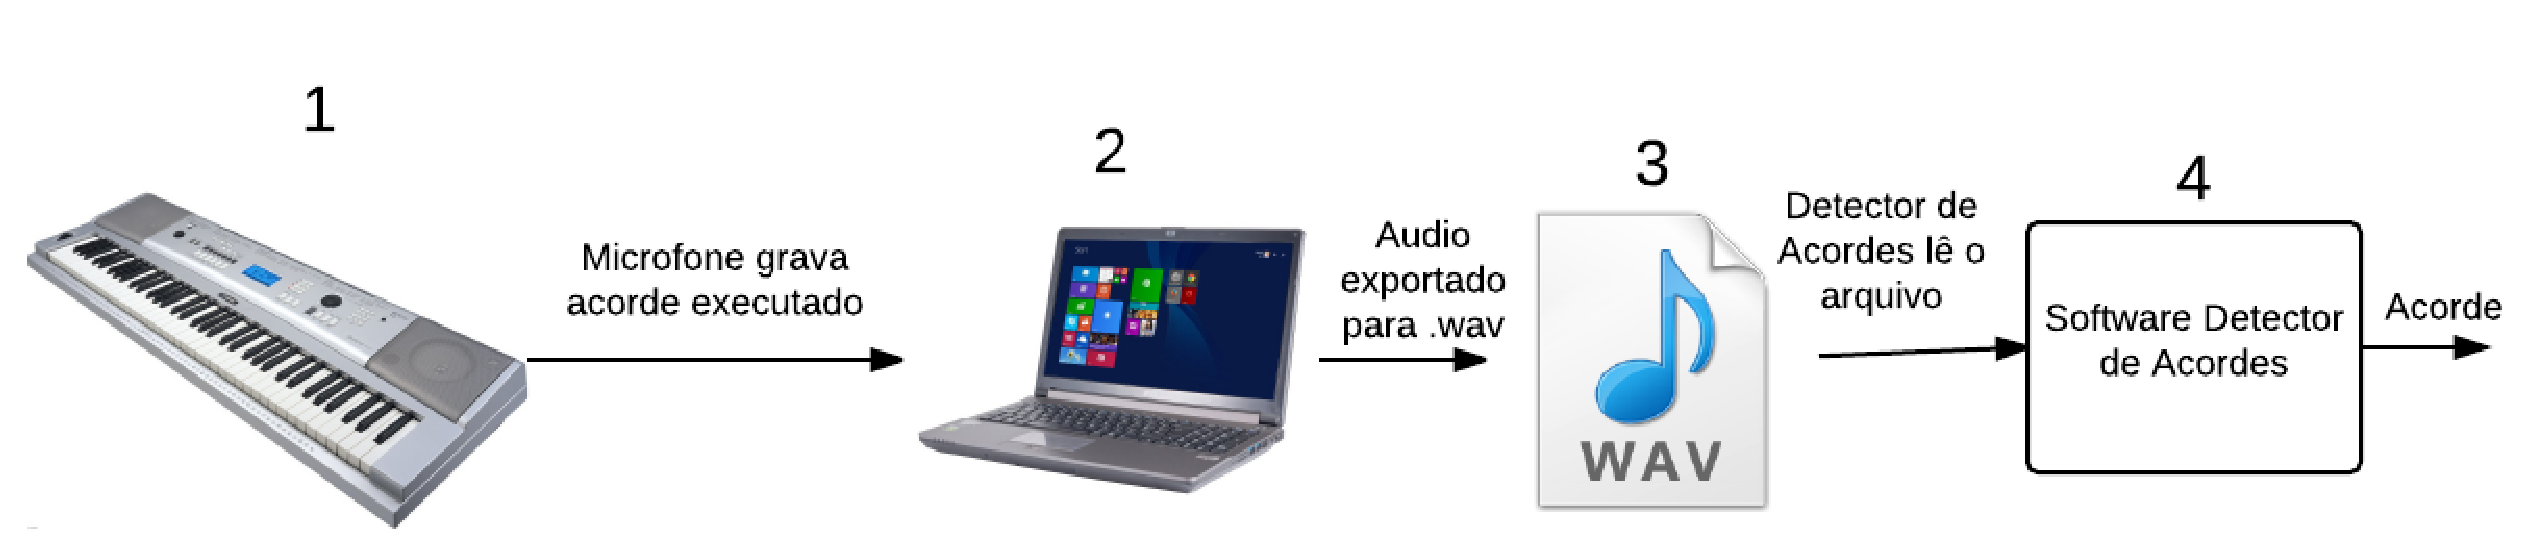
\includegraphics[keepaspectratio=true,scale=0.35]{figuras/processo_experimento.eps}
	\caption{Processo ilustrativo da execução dos experimentos}
\end{figure}

\newpage
\section{Experimento 1 - Acorde $CM$}
\label{sec:experimento1}

Nesse experimento foi tocado a tríade $Dó$ (baixo e tônica), $Mi$ e $Sol$ equivalente ao acorde $CM$. A tríade foi tocada ao mesmo tempo e com a mesma força para todas as notas.

Segue os gráficos resultantes:

\begin{figure}[h]
	\centering
		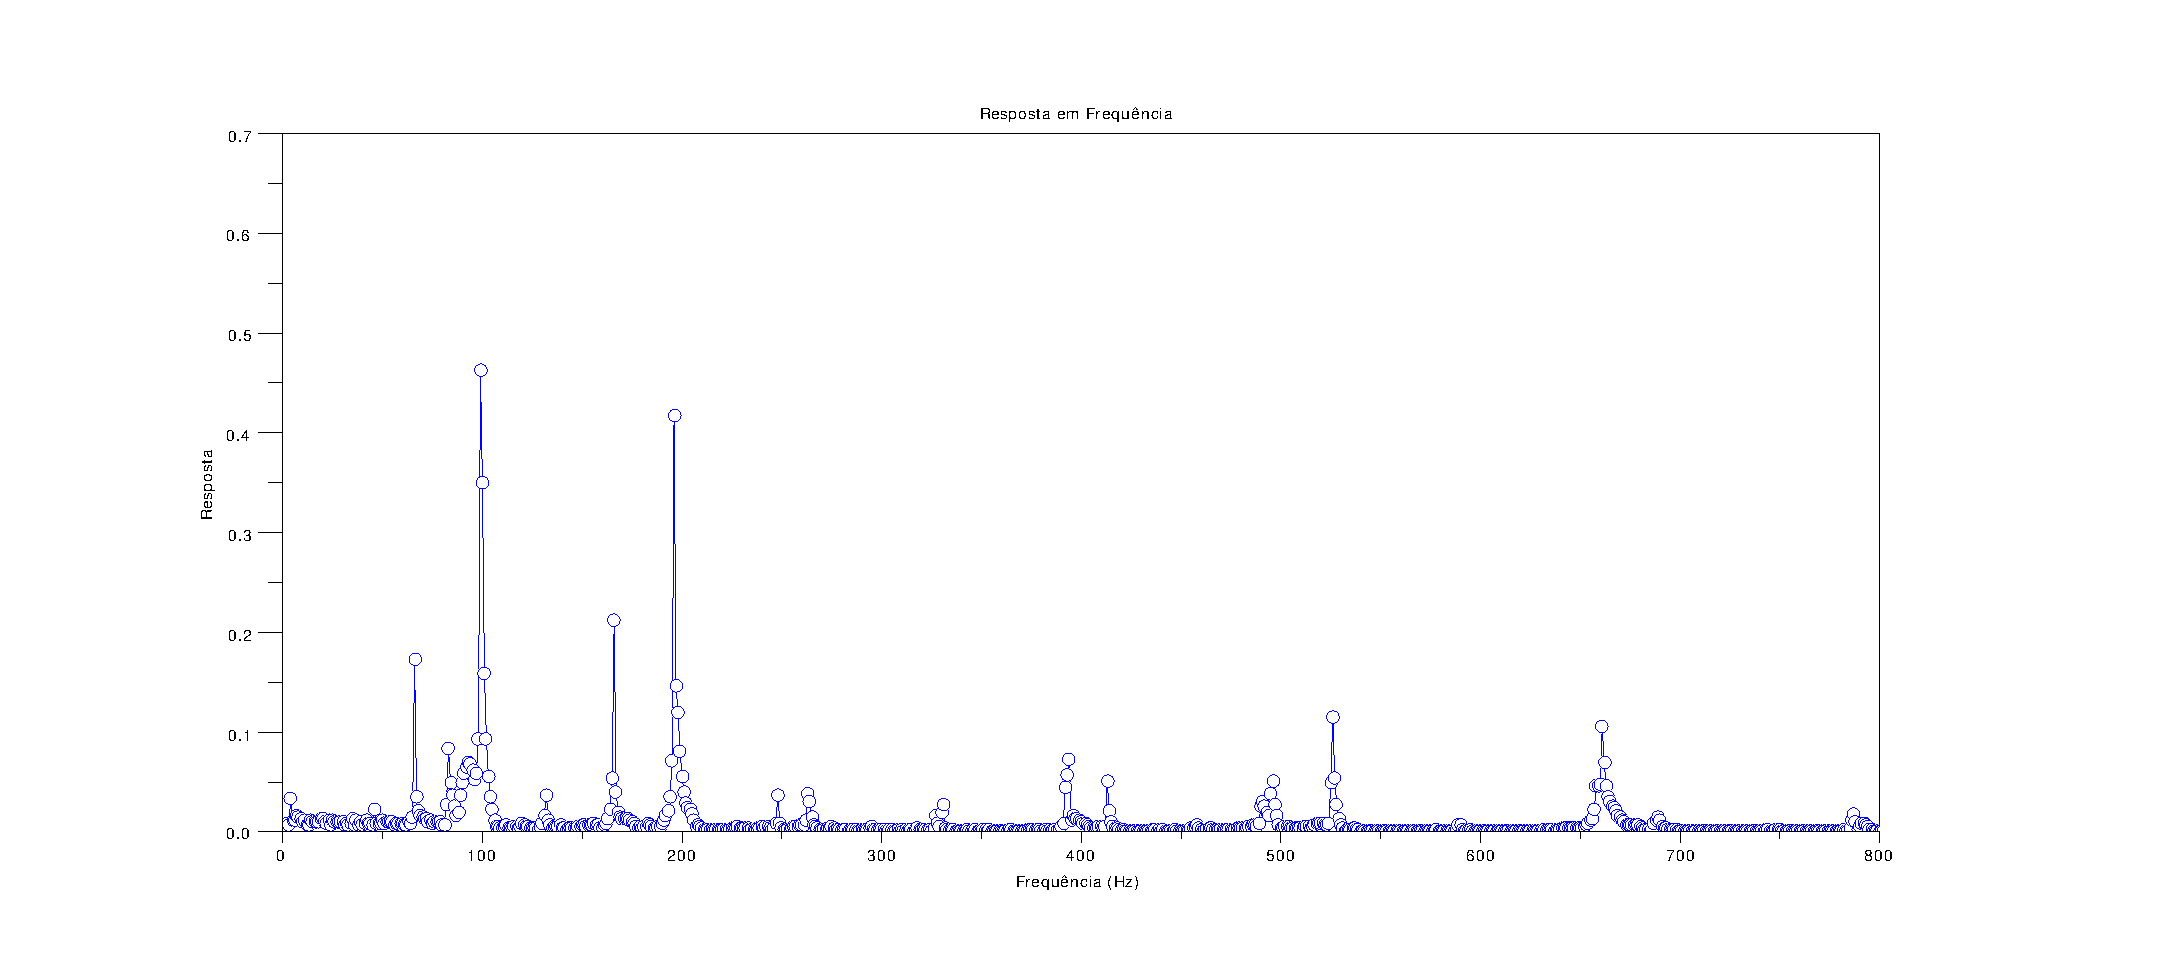
\includegraphics[keepaspectratio=true,scale=0.49]{figuras/CM/fft_cm.eps}
	\caption{Gráfico da resposta em frequência para a gravação do acorde $CM$}
\end{figure}

\begin{figure}[h]
	\centering
		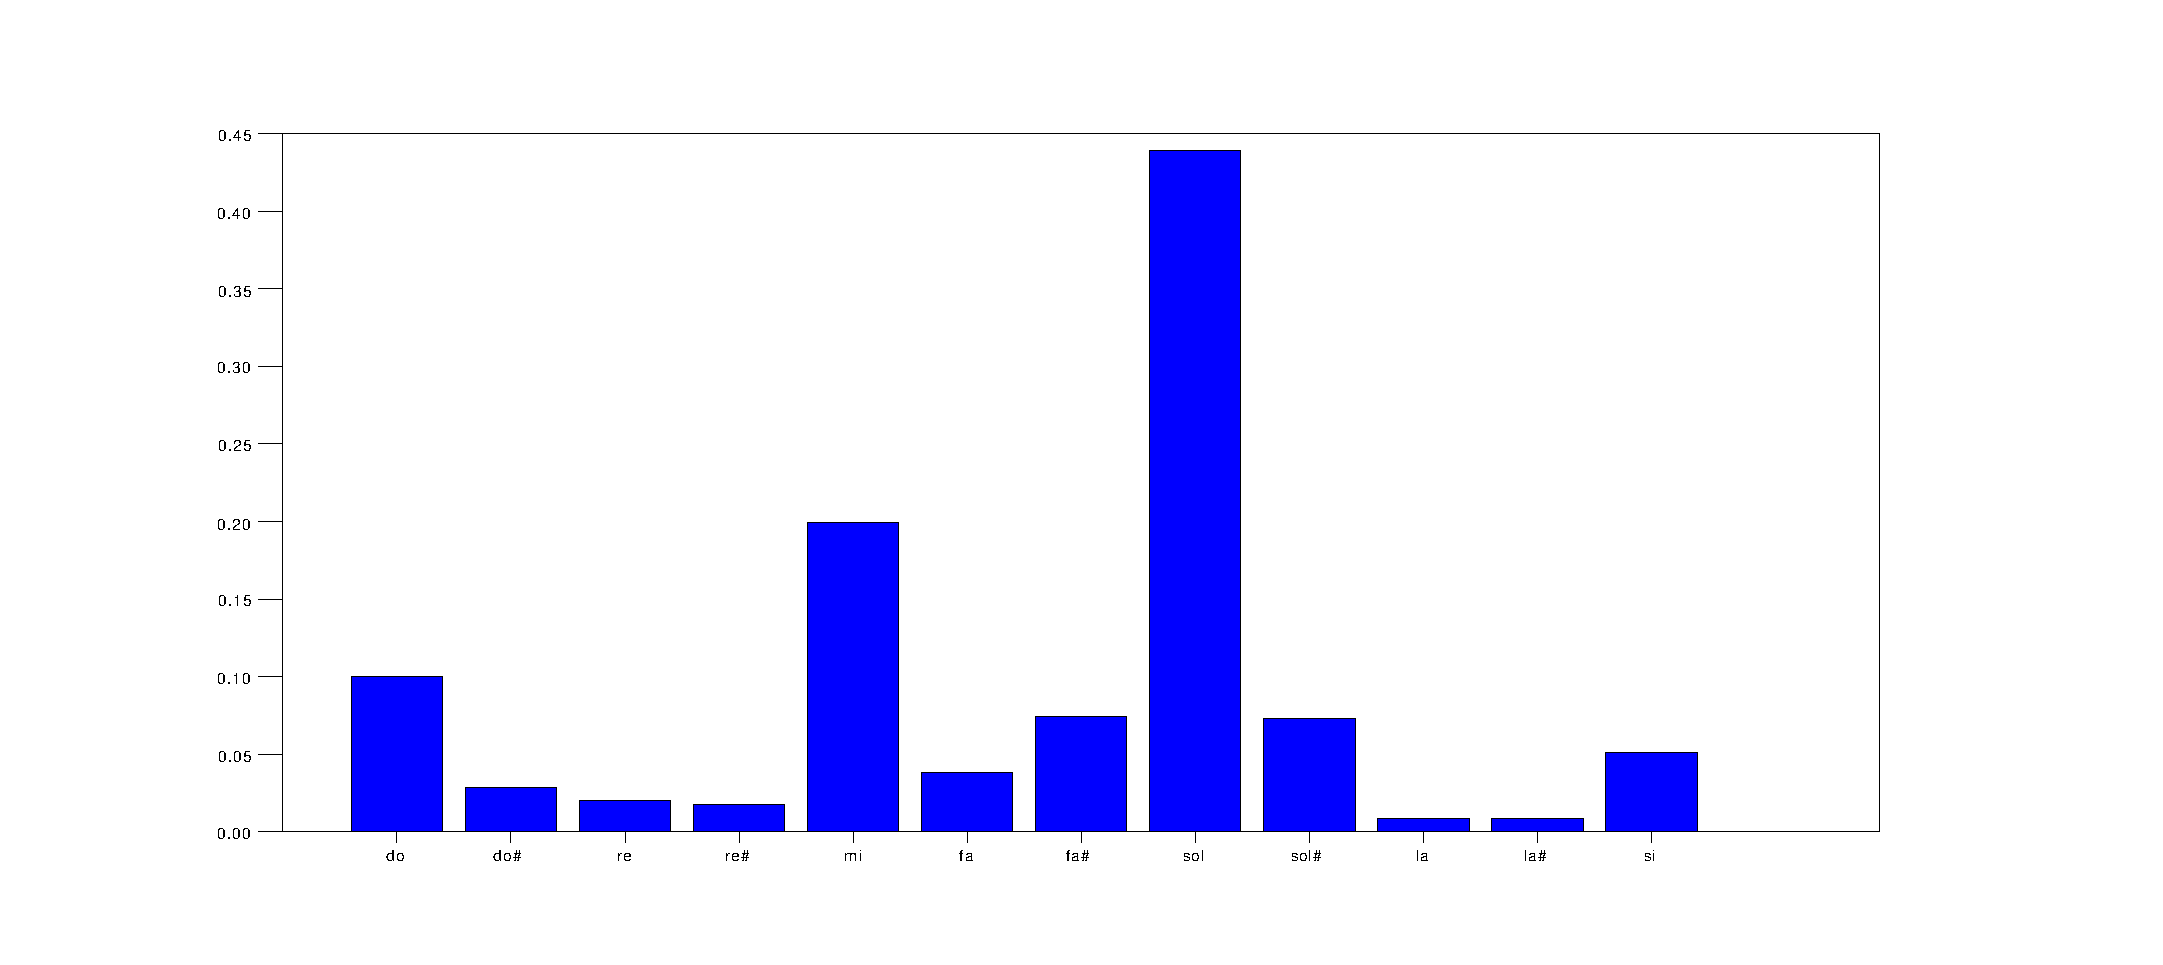
\includegraphics[keepaspectratio=true,scale=0.49]{figuras/CM/notas_cm.eps}
	\caption{Gráfico de sugestão de notas para a gravação do acorde $CM$}
\end{figure}

\begin{figure}[h]
	\centering
		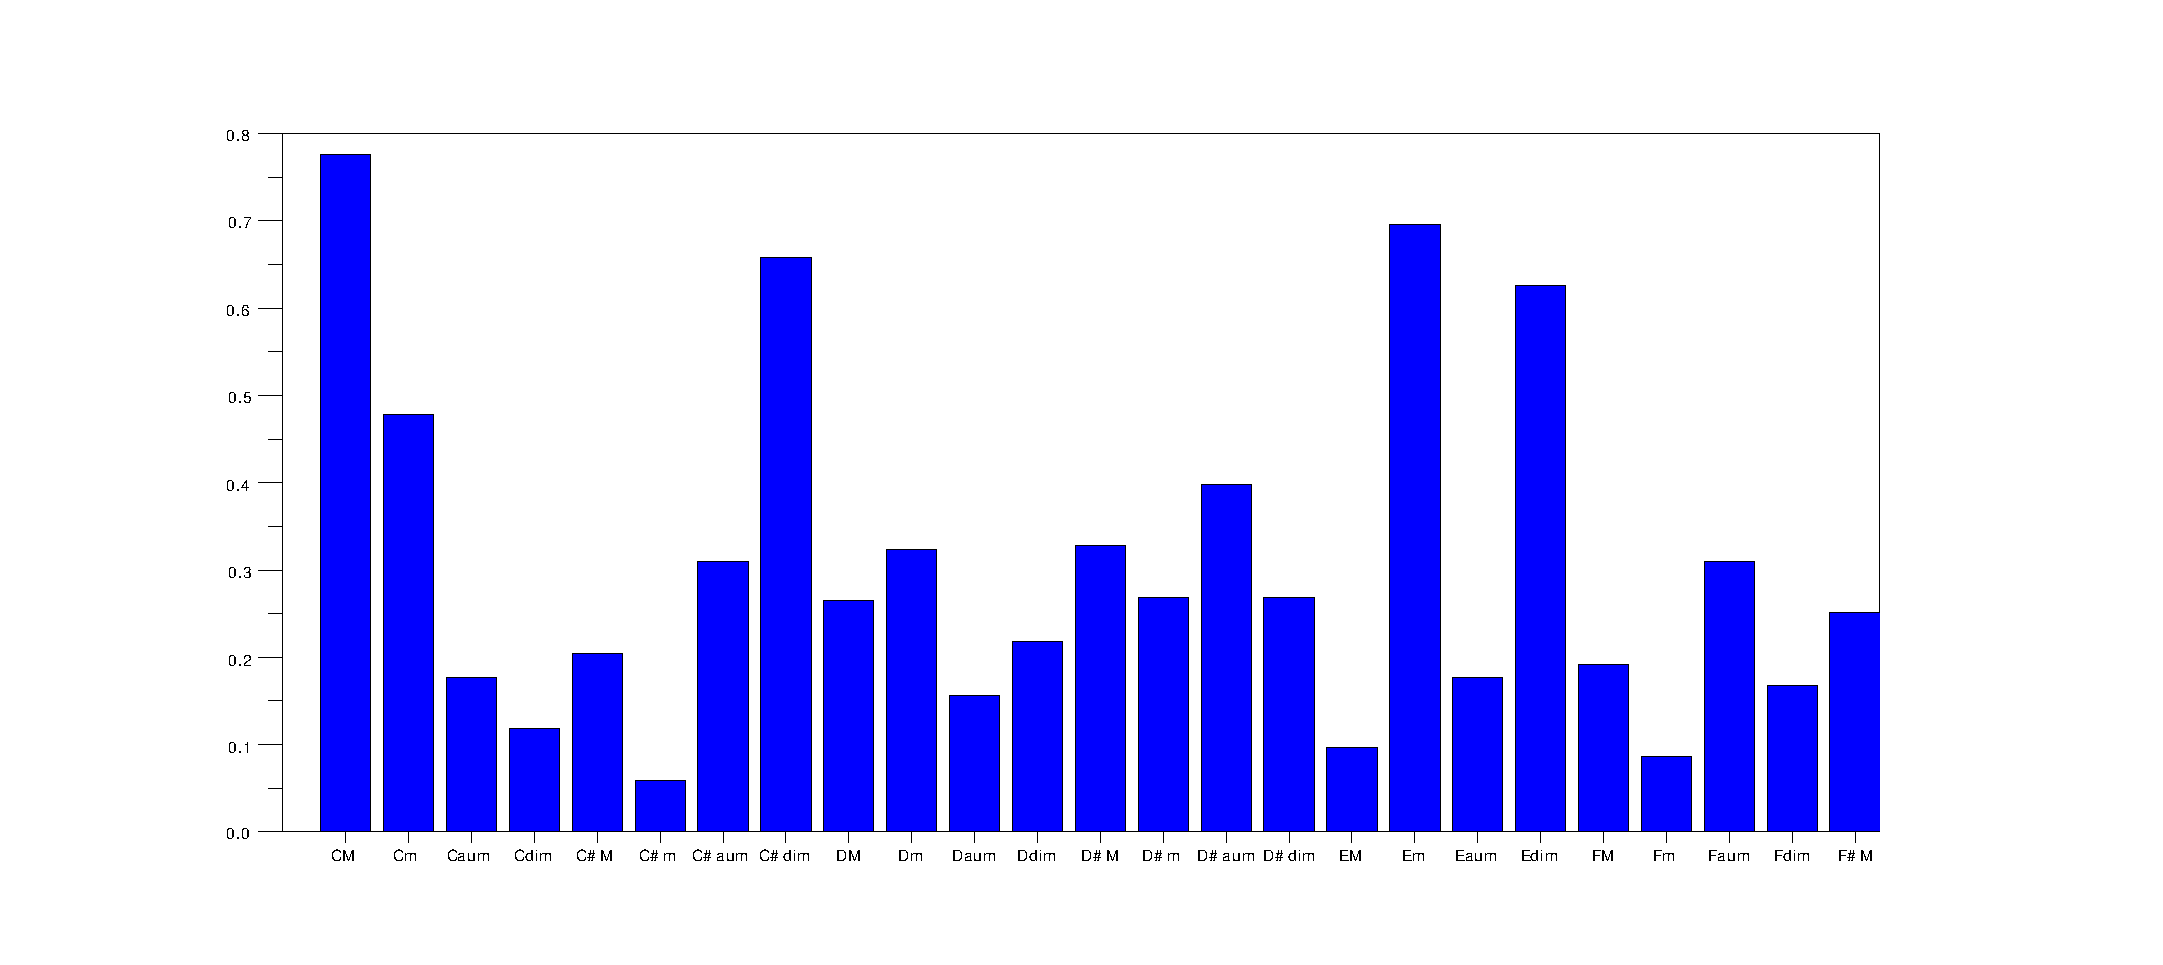
\includegraphics[keepaspectratio=true,scale=0.45]{figuras/CM/acordes_1_cm.eps}
		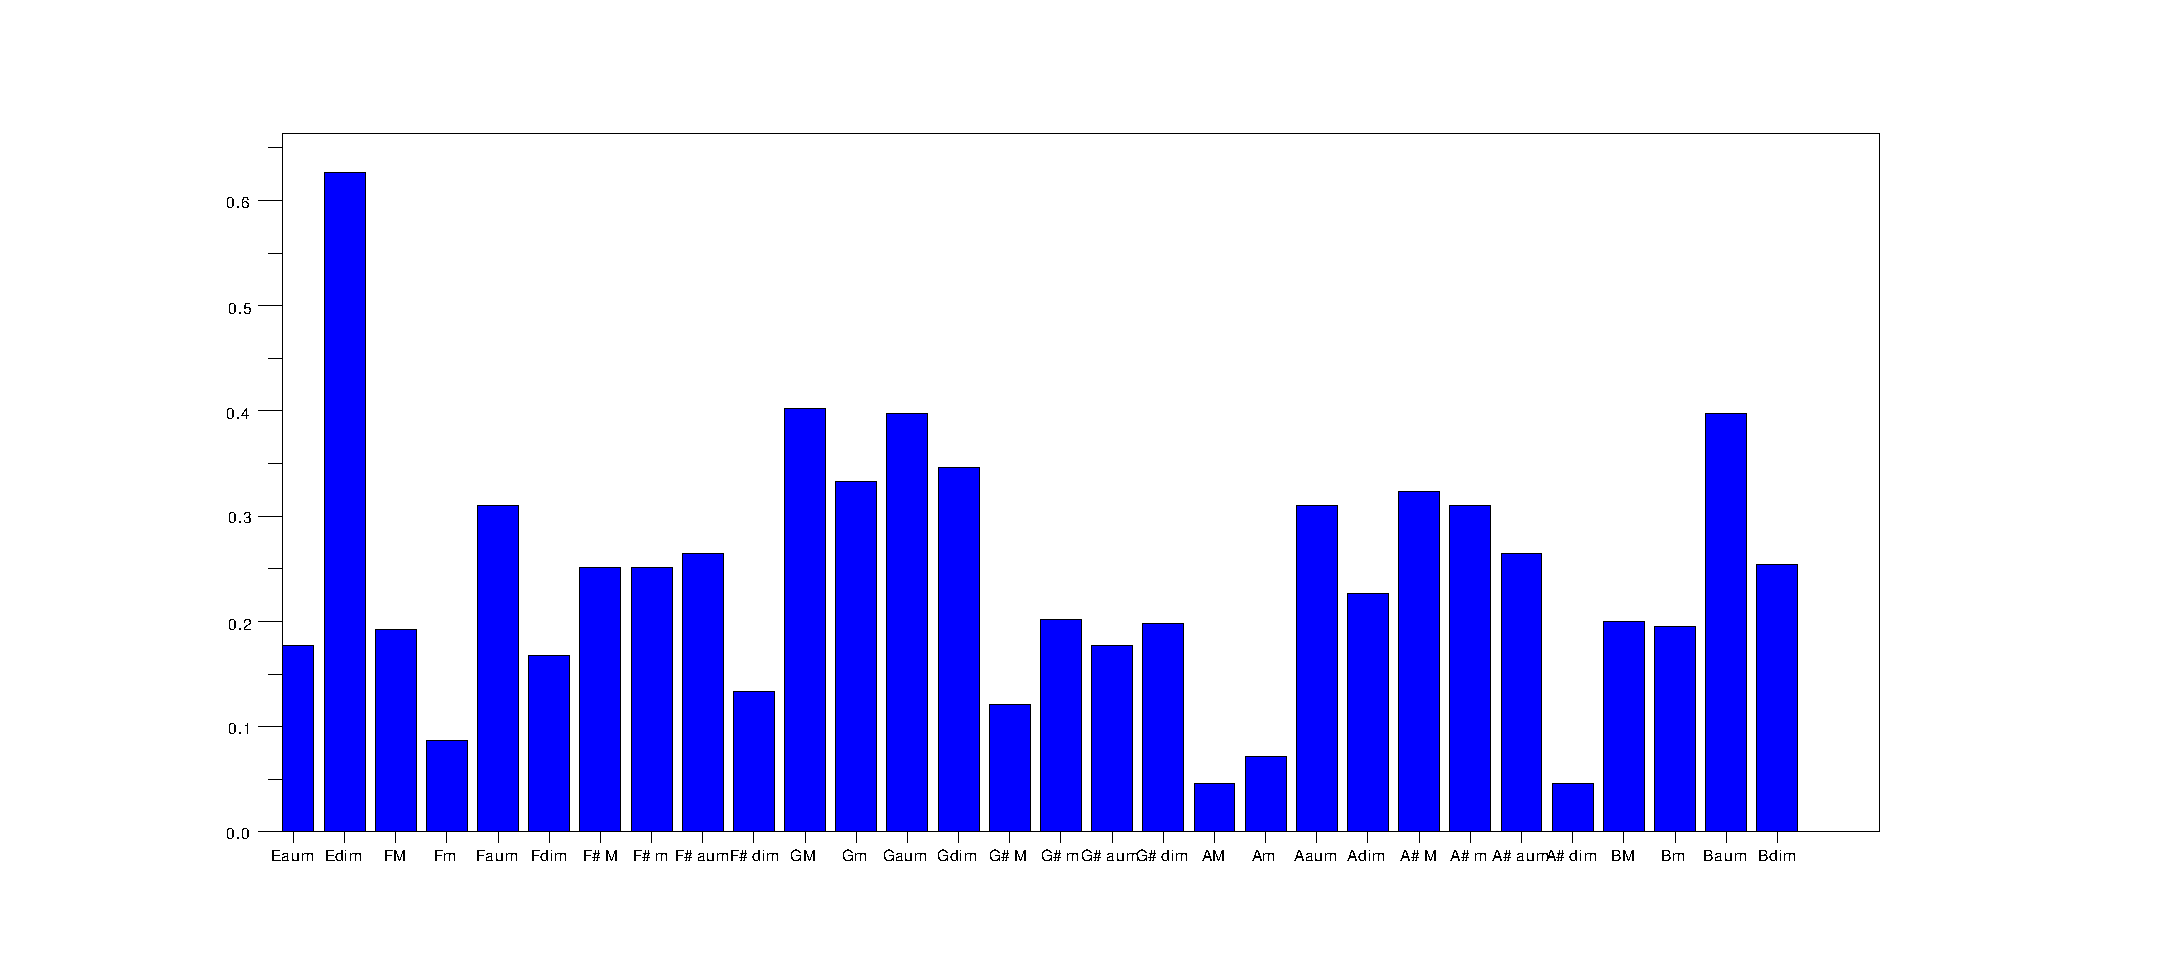
\includegraphics[keepaspectratio=true,scale=0.45]{figuras/CM/acordes_2_cm.eps}
	\caption{Gráficos de sugestão de acordes a gravação do acorde $CM$}
\end{figure}
\newpage
Do resultado da primeira camada de processamento é gerado o gráfico da Figura 16. Esse gráfico diz respeito a natureza da composição do sinal em senoides em termos de transformada de fourier. O primeiro pico, no valor de 294 Hz, é relativo a nota $Dó$. O segundo pico, no valor de 371 Hz, é relativo a nota $Mi$. O terceiro pico, no valor de 441 Hz, é relativo a nota $Sol$. Os picos seguintes são relativos aos harmônicos dessas três notas.

Do resultado da segunda camada de processamento é gerado gráfico da Figura 17. É possível perceber nele que as notas $Dó$, $Mi$ e $Sol$ são as que mais possuem energia ou, no ponto de vista de sugestão, as mais sugeridas. De certa forma um dos fatores que contribuiram das notas $Dó$ e $Sol$ ser de maiores energias foi devido a presença dos harmônicos.

Do resultado da terceira camada de processamento são gerados os gráficos da Figura 18. Essa camada é relativa ao resultados das sugestões de acordes musicais. É perceptível ver a presença da alta sugestão do acorde $CM$.
\section{Experimento 2 - Acorde $Dm$}
\label{sec:experimento2}

Nesse experimento foi tocado a tríade $Ré$ (baixo e tônica), $Fá$ e $Lá$ equivalente ao acorde $Dm$. A tríade foi tocada ao mesmo tempo e com a mesma força para todas as notas.

Segue os gráficos resultantes:

\begin{figure}[h]
	\centering
		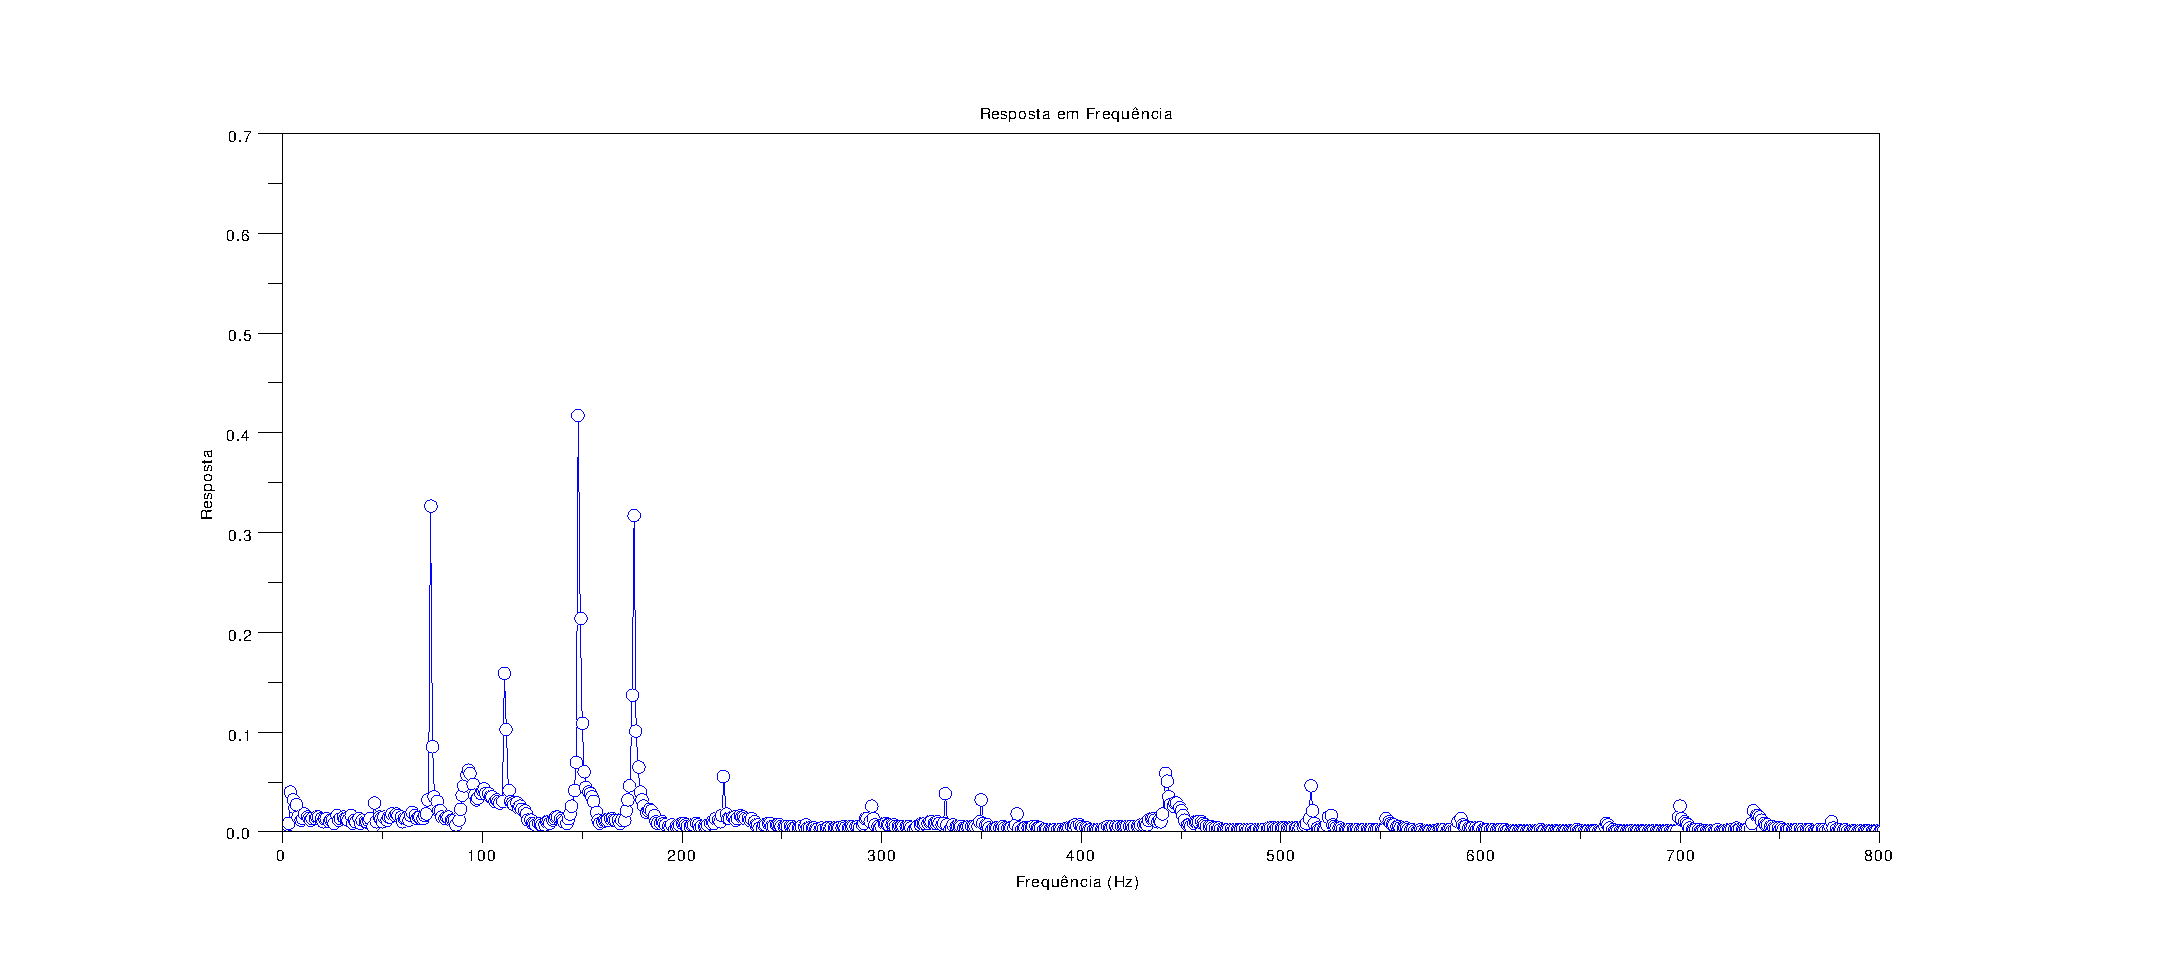
\includegraphics[keepaspectratio=true,scale=0.49]{figuras/Dm/fft_Dm.eps}
	\caption{Gráfico da resposta em frequência para a gravação do acorde $Dm$}
\end{figure}

\begin{figure}[h]
	\centering
		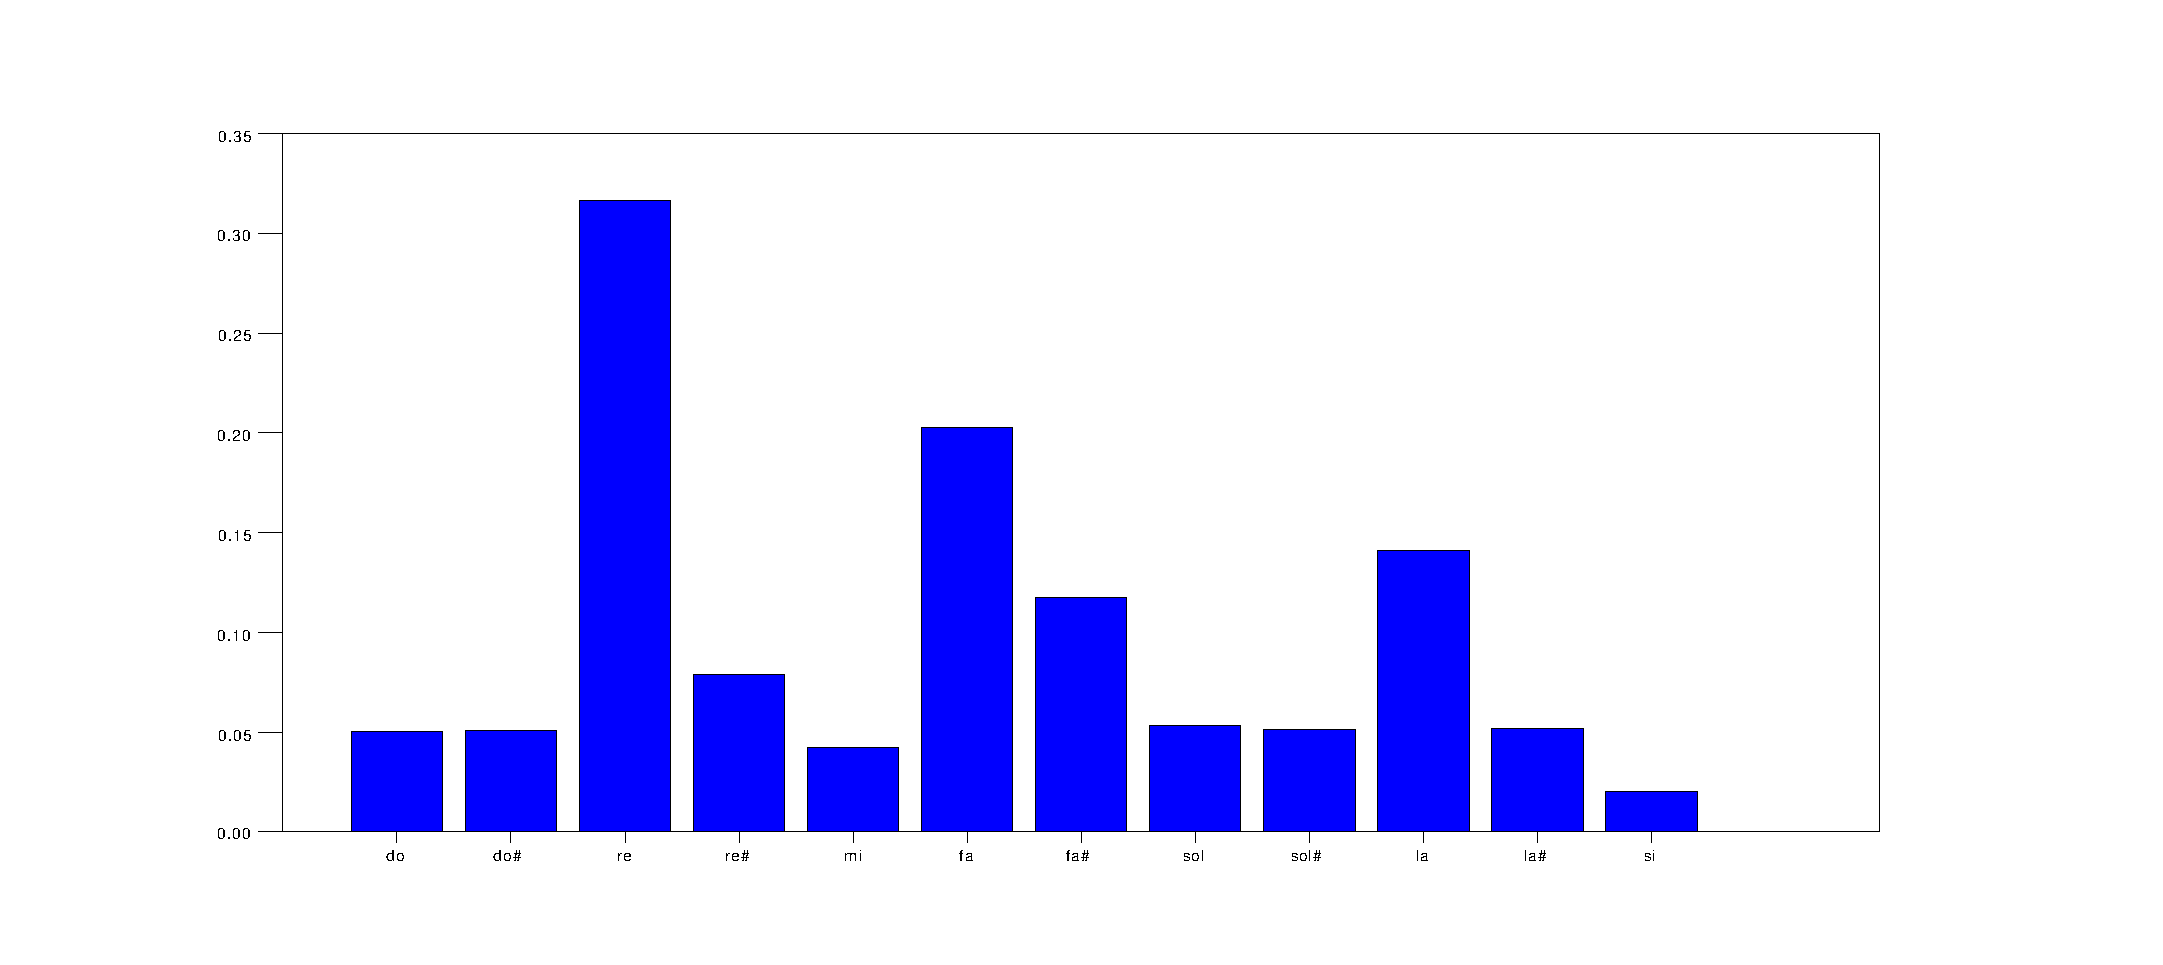
\includegraphics[keepaspectratio=true,scale=0.49]{figuras/Dm/notas_Dm.eps}
	\caption{Gráfico de sugestão de notas para a gravação do acorde $Dm$}
\end{figure}

\begin{figure}[h]
	\centering
		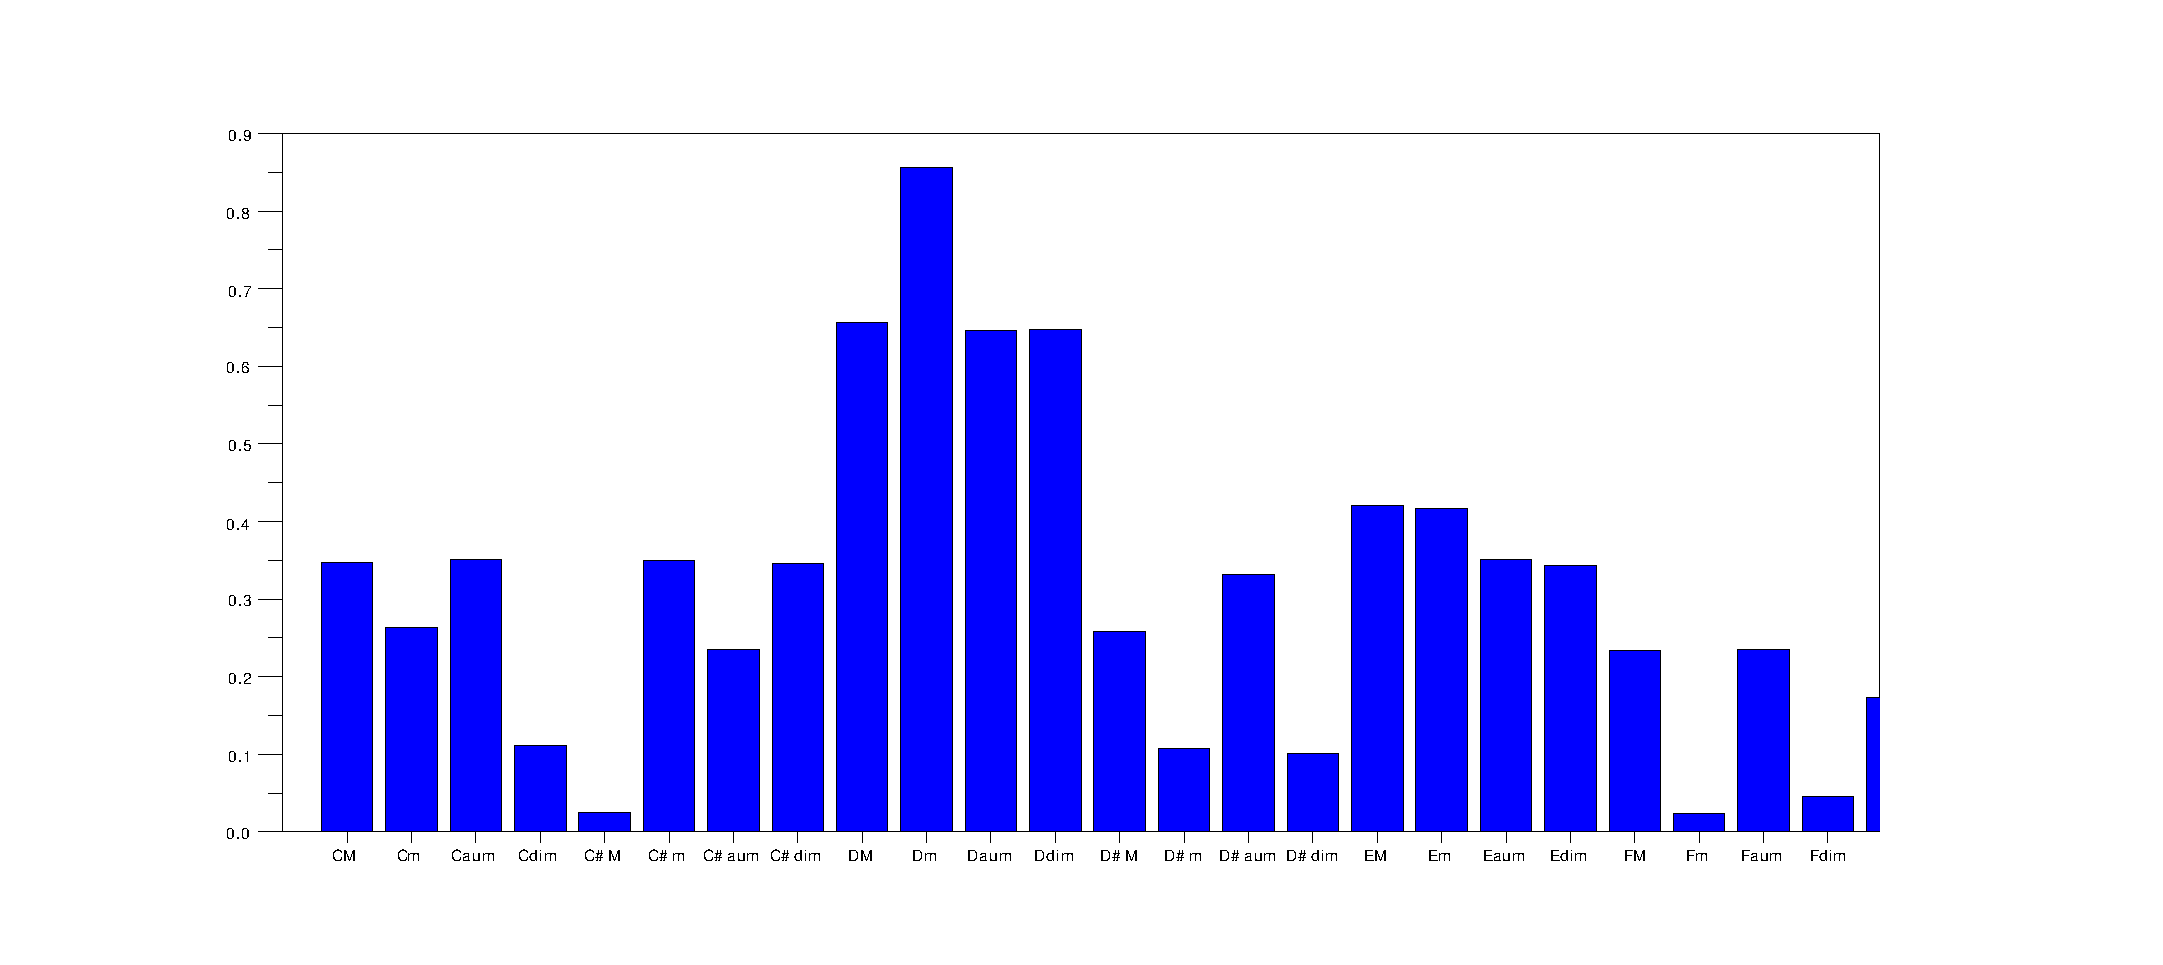
\includegraphics[keepaspectratio=true,scale=0.49]{figuras/Dm/acordes_1_Dm.eps}
		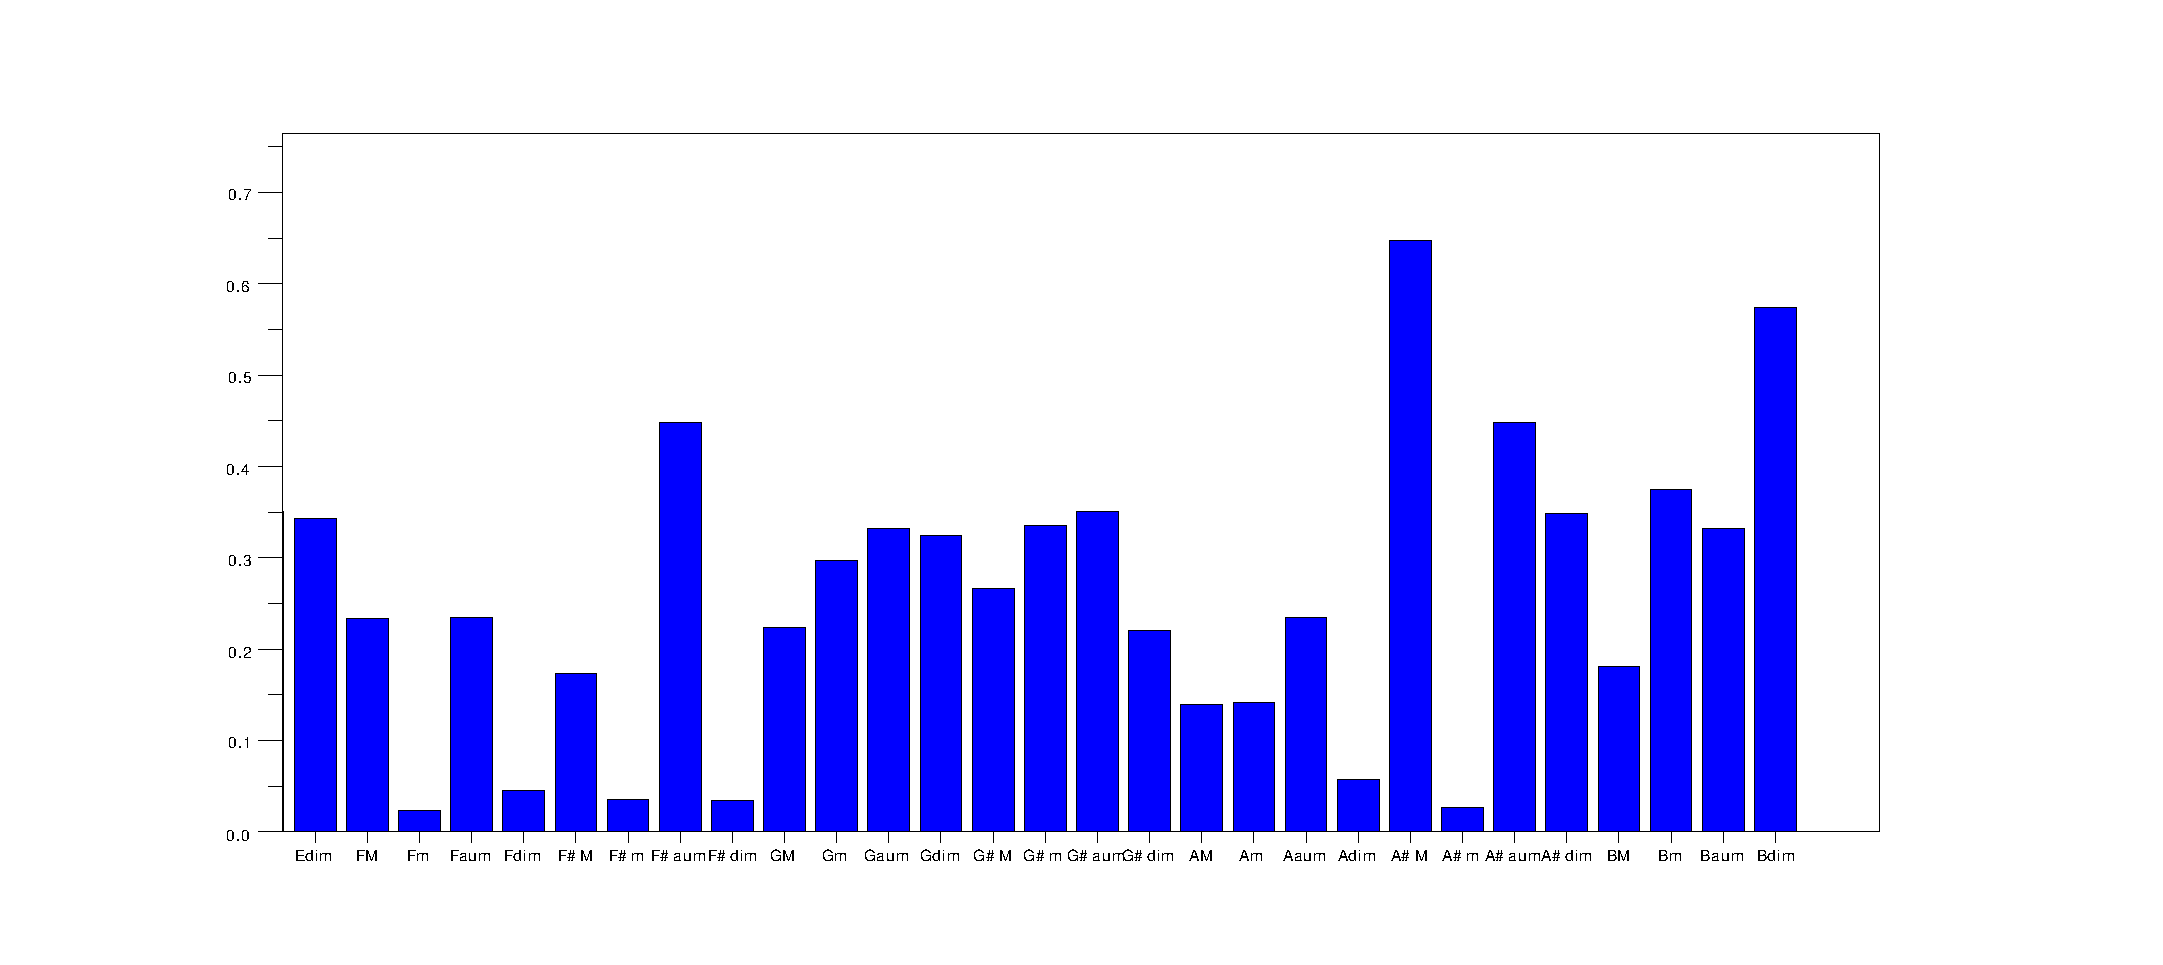
\includegraphics[keepaspectratio=true,scale=0.49]{figuras/Dm/acordes_2_Dm.eps}
	\caption{Gráficos de sugestão de acordes a gravação do acorde $Dm$}
\end{figure}
\newpage

Do resultado da primeira camada de processamento é gerado o gráfico da Figura 19. Esse gráfico diz respeito a natureza da composição do sinal em senoides em termos de transformada de fourier. O primeiro pico, no valor de 294 Hz, é relativo a nota $Ré$. O segundo pico, no valor de 350 Hz, é relativo a nota $Fá$. O terceiro pico, no valor de 441 Hz, é relativo a nota $Lá$. Os picos seguintes são relativos aos harmônicos dessas três notas.

Do resultado da segunda camada de processamento é gerado gráfico da Figura 20. É possível perceber nele que as notas $Ré$, $Fá$ e $Lá$ são as que mais possuem energia ou, no ponto de vista de sugestão, as mais sugeridas. De certa forma um dos fatores que contribuiram das notas $Ré$ e $Lá$ ser de maiores energias foi devido a presença dos harmônicos.

Do resultado da terceira camada de processamento são gerados os gráficos da Figura 21. Essa camada é relativa ao resultados das sugestões de acordes musicais. É perceptível ver a presença da alta sugestão do acorde $Dm$.

\section{Experimento 3 - Acorde $Ddim$}
\label{sec:experimento3}

Nesse experimento foi tocado a tríade $Ré$ (baixo e tônica), $Fá$ e $Sol\#$ equivalente ao acorde Ddim. A tríade foi tocada ao mesmo tempo e com a mesma força para todas as notas.

Segue os gráficos resultantes:

\begin{figure}[h]
	\centering
		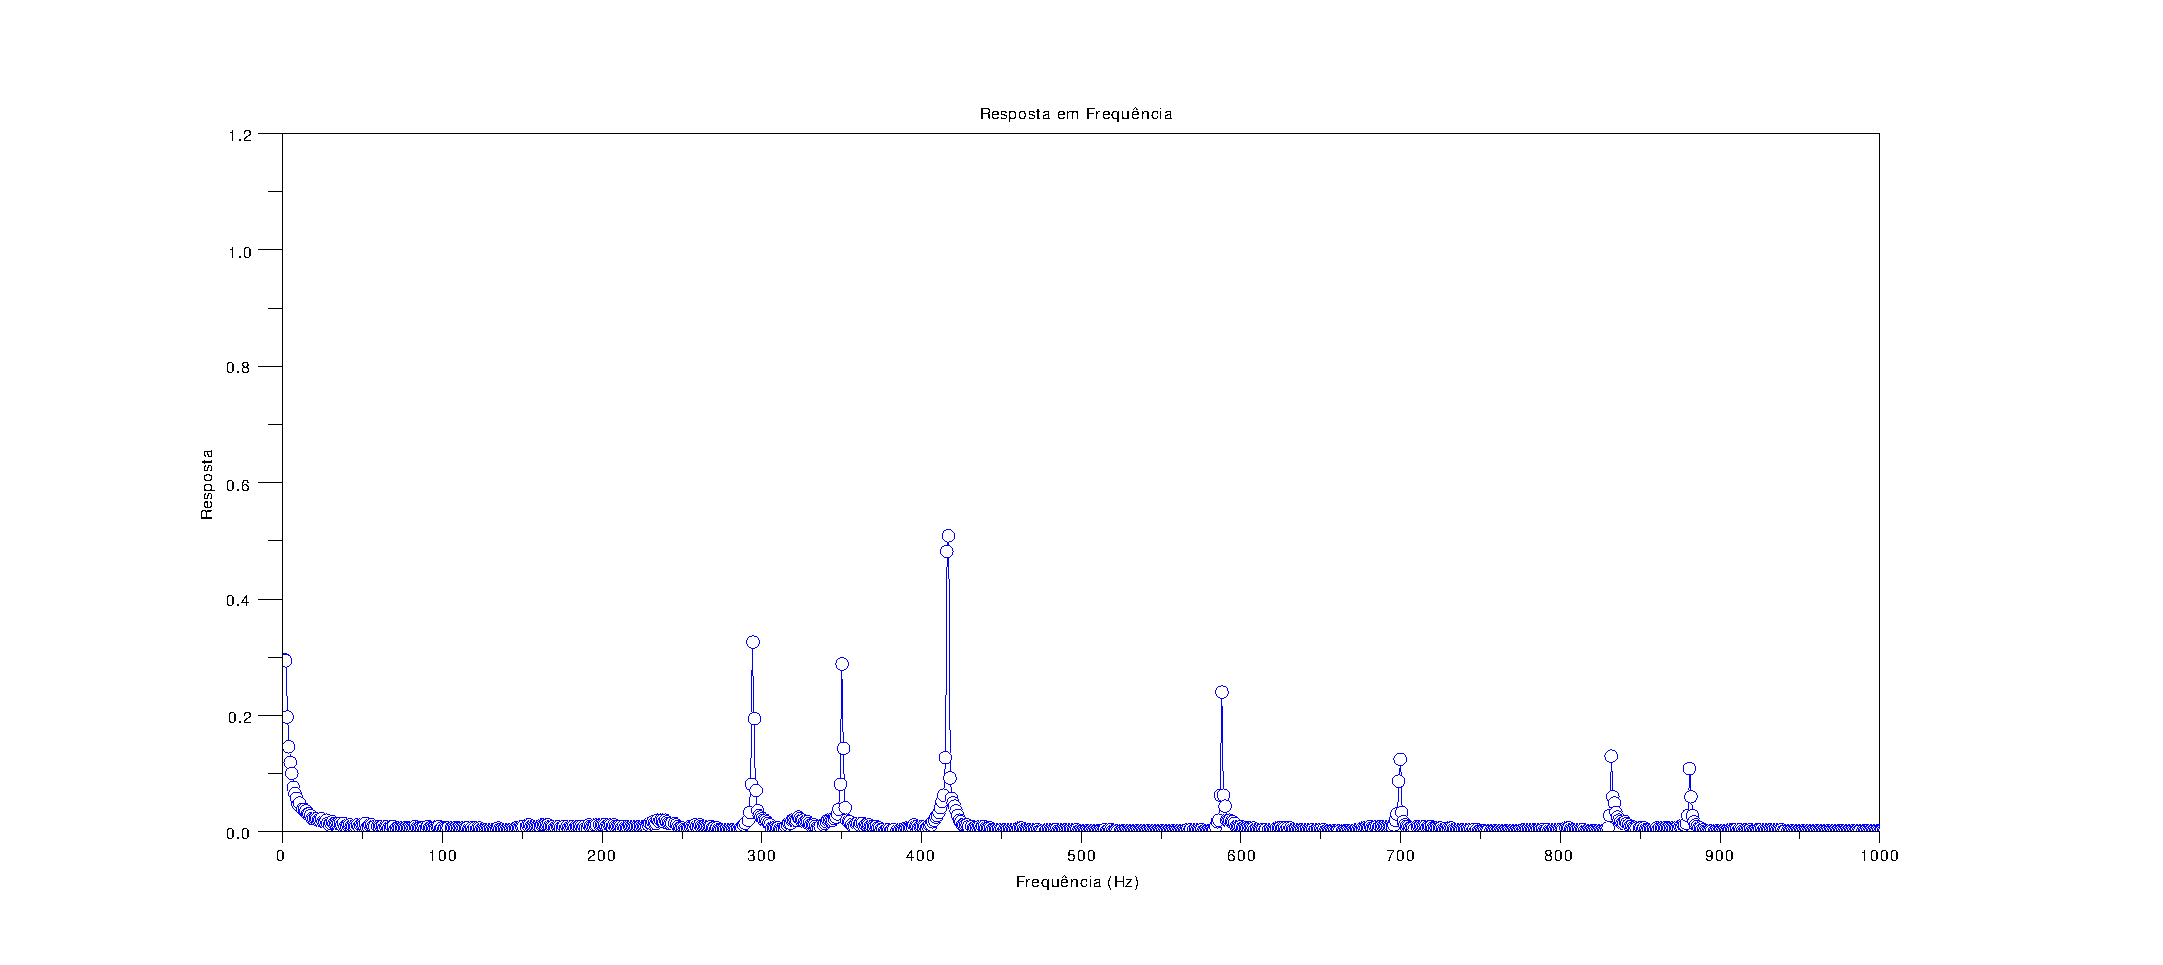
\includegraphics[keepaspectratio=true,scale=0.49]{figuras/Dm/fft_Ddim.eps}
	\caption{Gráfico da resposta em frequência para a gravação do acorde $Ddim$}
\end{figure}

\begin{figure}[h]
	\centering
		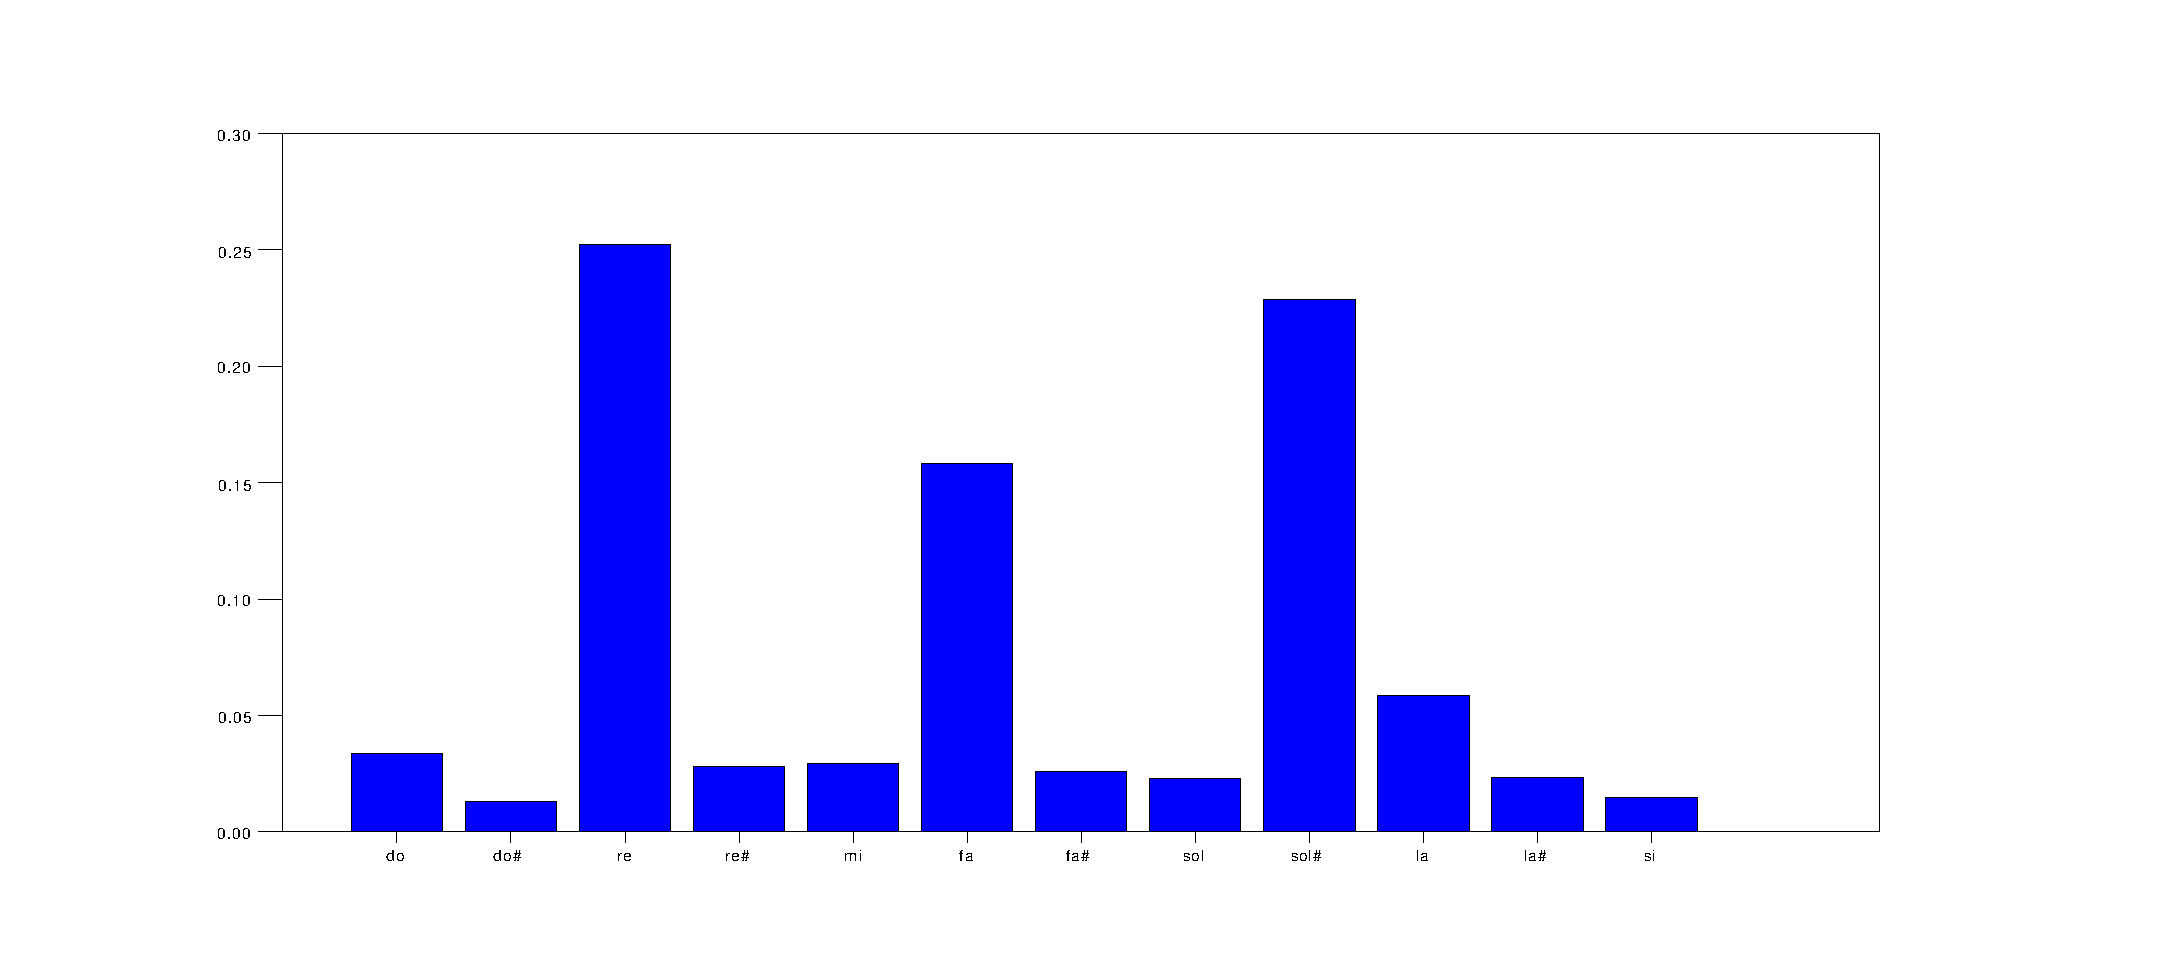
\includegraphics[keepaspectratio=true,scale=0.45]{figuras/Dm/notas_Ddim.eps}
	\caption{Gráfico de sugestão de notas para a gravação do acorde $Ddim$}
\end{figure}

\begin{figure}[h]
	\centering
		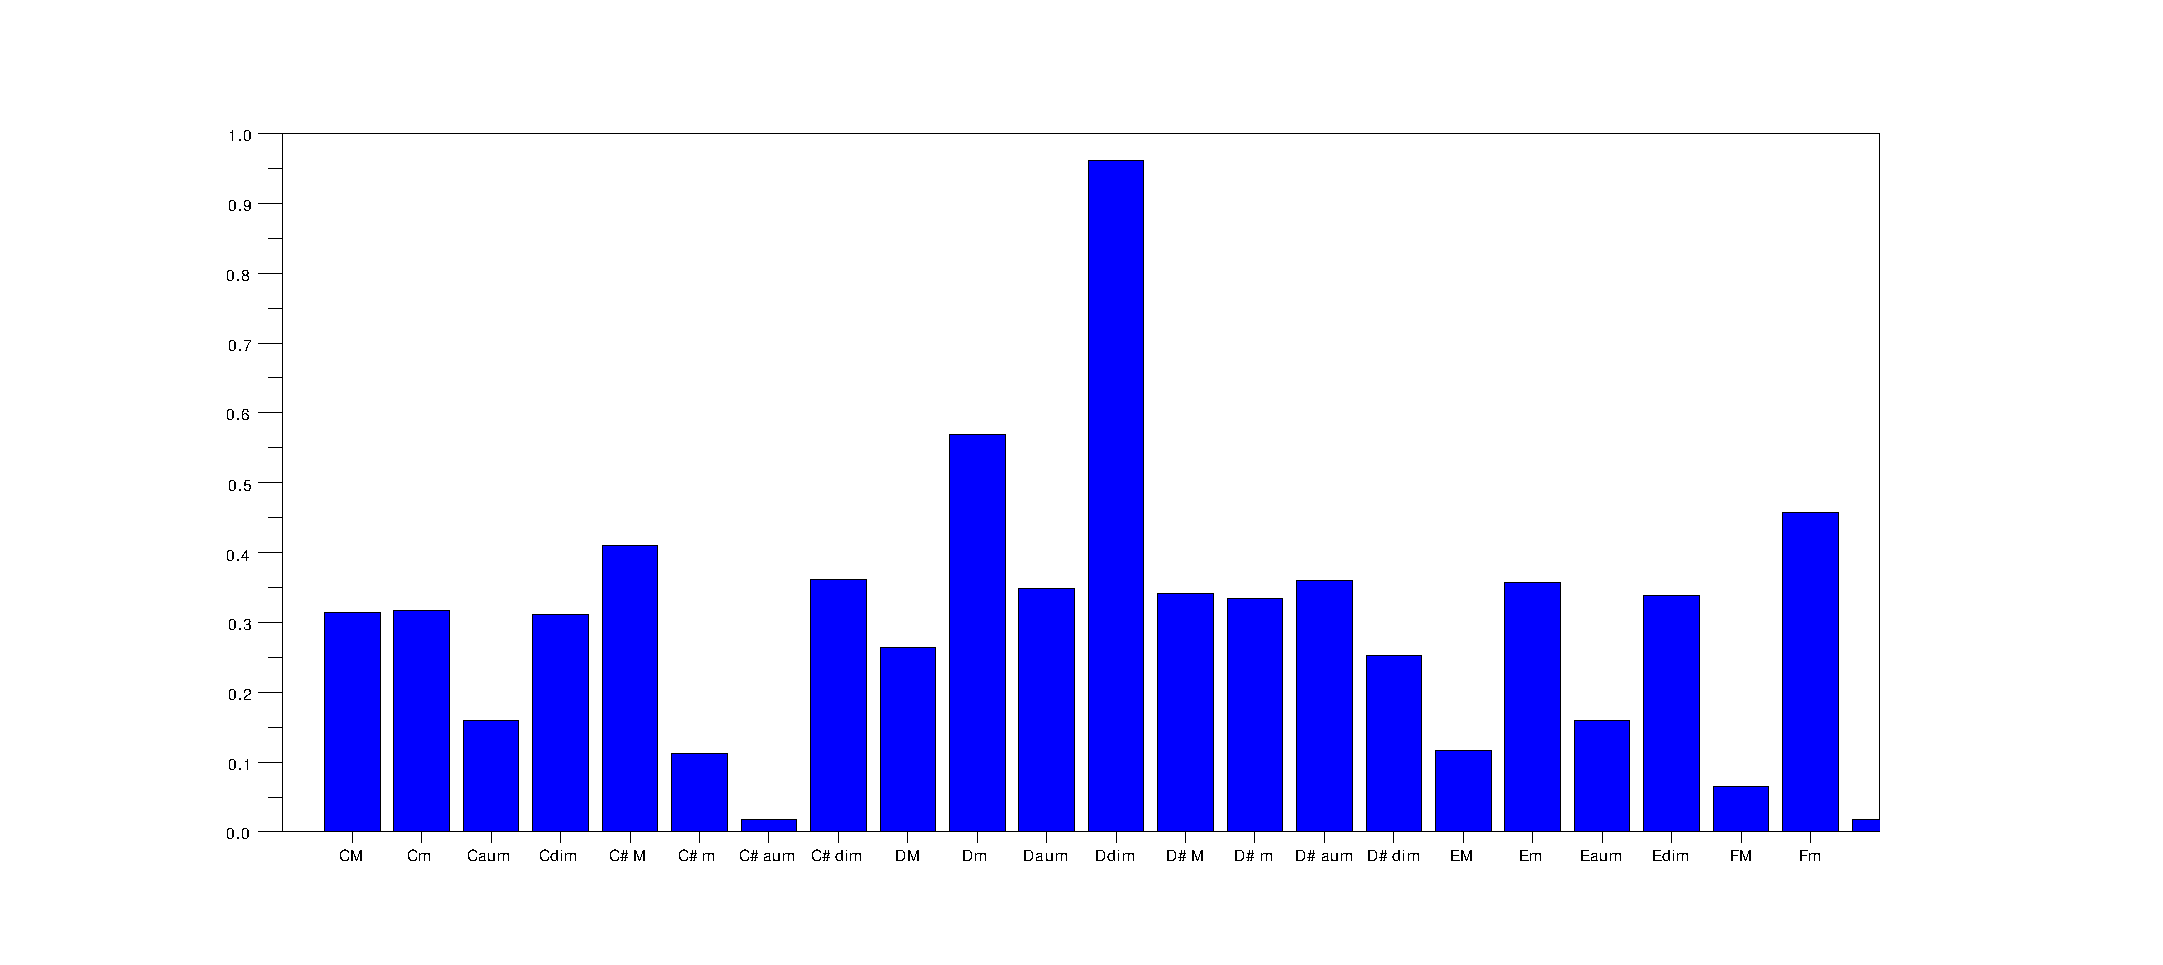
\includegraphics[keepaspectratio=true,scale=0.49]{figuras/Dm/acordes_1_Ddim.eps}
		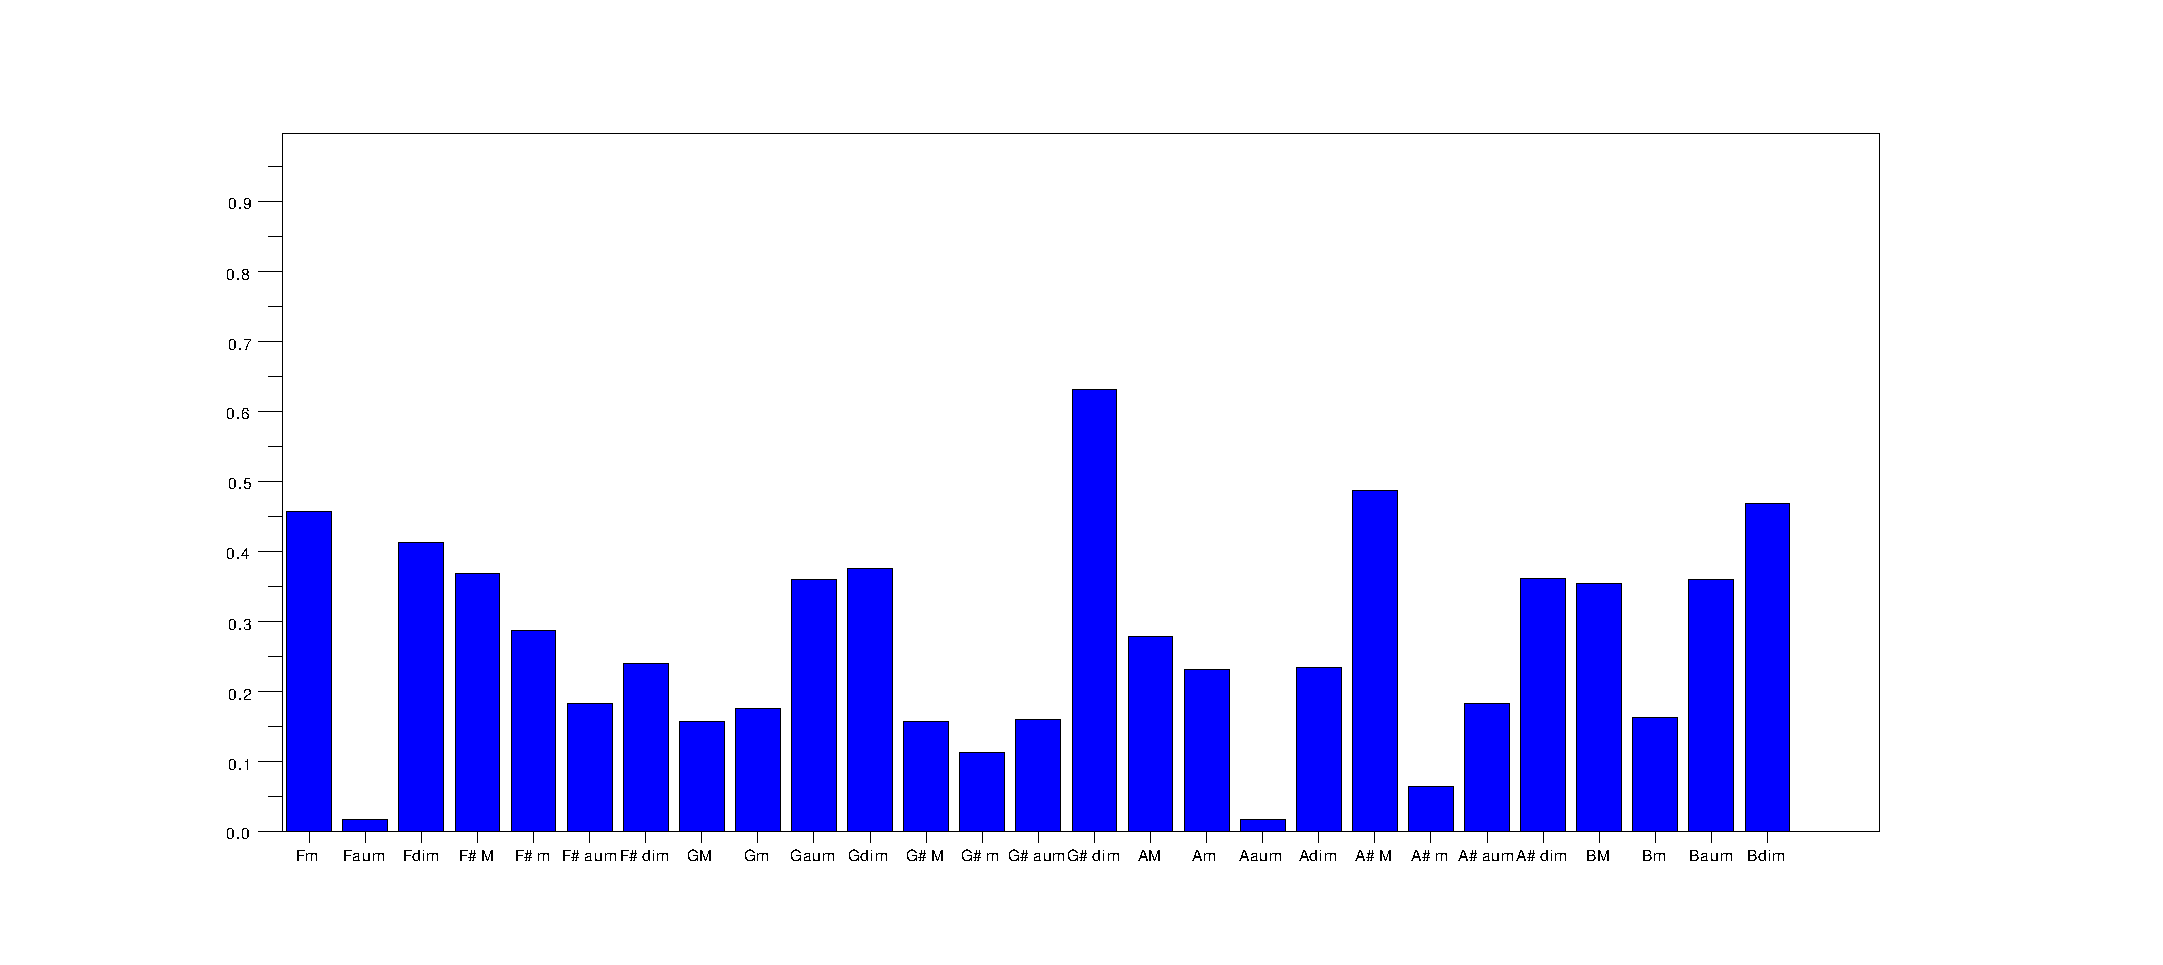
\includegraphics[keepaspectratio=true,scale=0.49]{figuras/Dm/acordes_2_Ddim.eps}
	\caption{Gráficos de sugestão de acordes a gravação do acorde $Ddim$}
\end{figure}
\newpage

Do resultado da primeira camada de processamento é gerado o gráfico da Figura 22. Esse gráfico diz respeito a natureza da composição do sinal em senoides em termos de transformada de fourier. O primeiro pico, no valor de 294 Hz, é relativo a nota $Ré$. O segundo pico, no valor de 350 Hz, é relativo a nota $Fá$. O terceiro pico, no valor de 417 Hz, é relativo a nota $Sol\#$. Os picos seguintes são relativos aos harmônicos dessas três notas.

Do resultado da segunda camada de processamento é gerado gráfico da Figura 23. É possível perceber nele que as notas $Ré$, $Fá$ e $Sol\#$ são as que mais possuem energia ou, no ponto de vista de sugestão, as mais sugeridas.

Do resultado da terceira camada de processamento são gerados os gráficos da Figura 24. Essa camada é relativa ao resultados das sugestões de acordes musicais. É perceptível ver a presença da alta sugestão do acorde $Ddim$.

\section{Experimento 4 - Acorde $Daum$}
\label{sec:experimento4}

Nesse experimento foi tocado a tríade $Ré$ (baixo e tônica), $Fá\#$ e $Lá\#$ equivalente ao acorde $Daum$. A tríade foi tocada ao mesmo tempo e com a mesma força para todas as notas.

Segue os gráficos resultantes:

\begin{figure}[h]
	\centering
		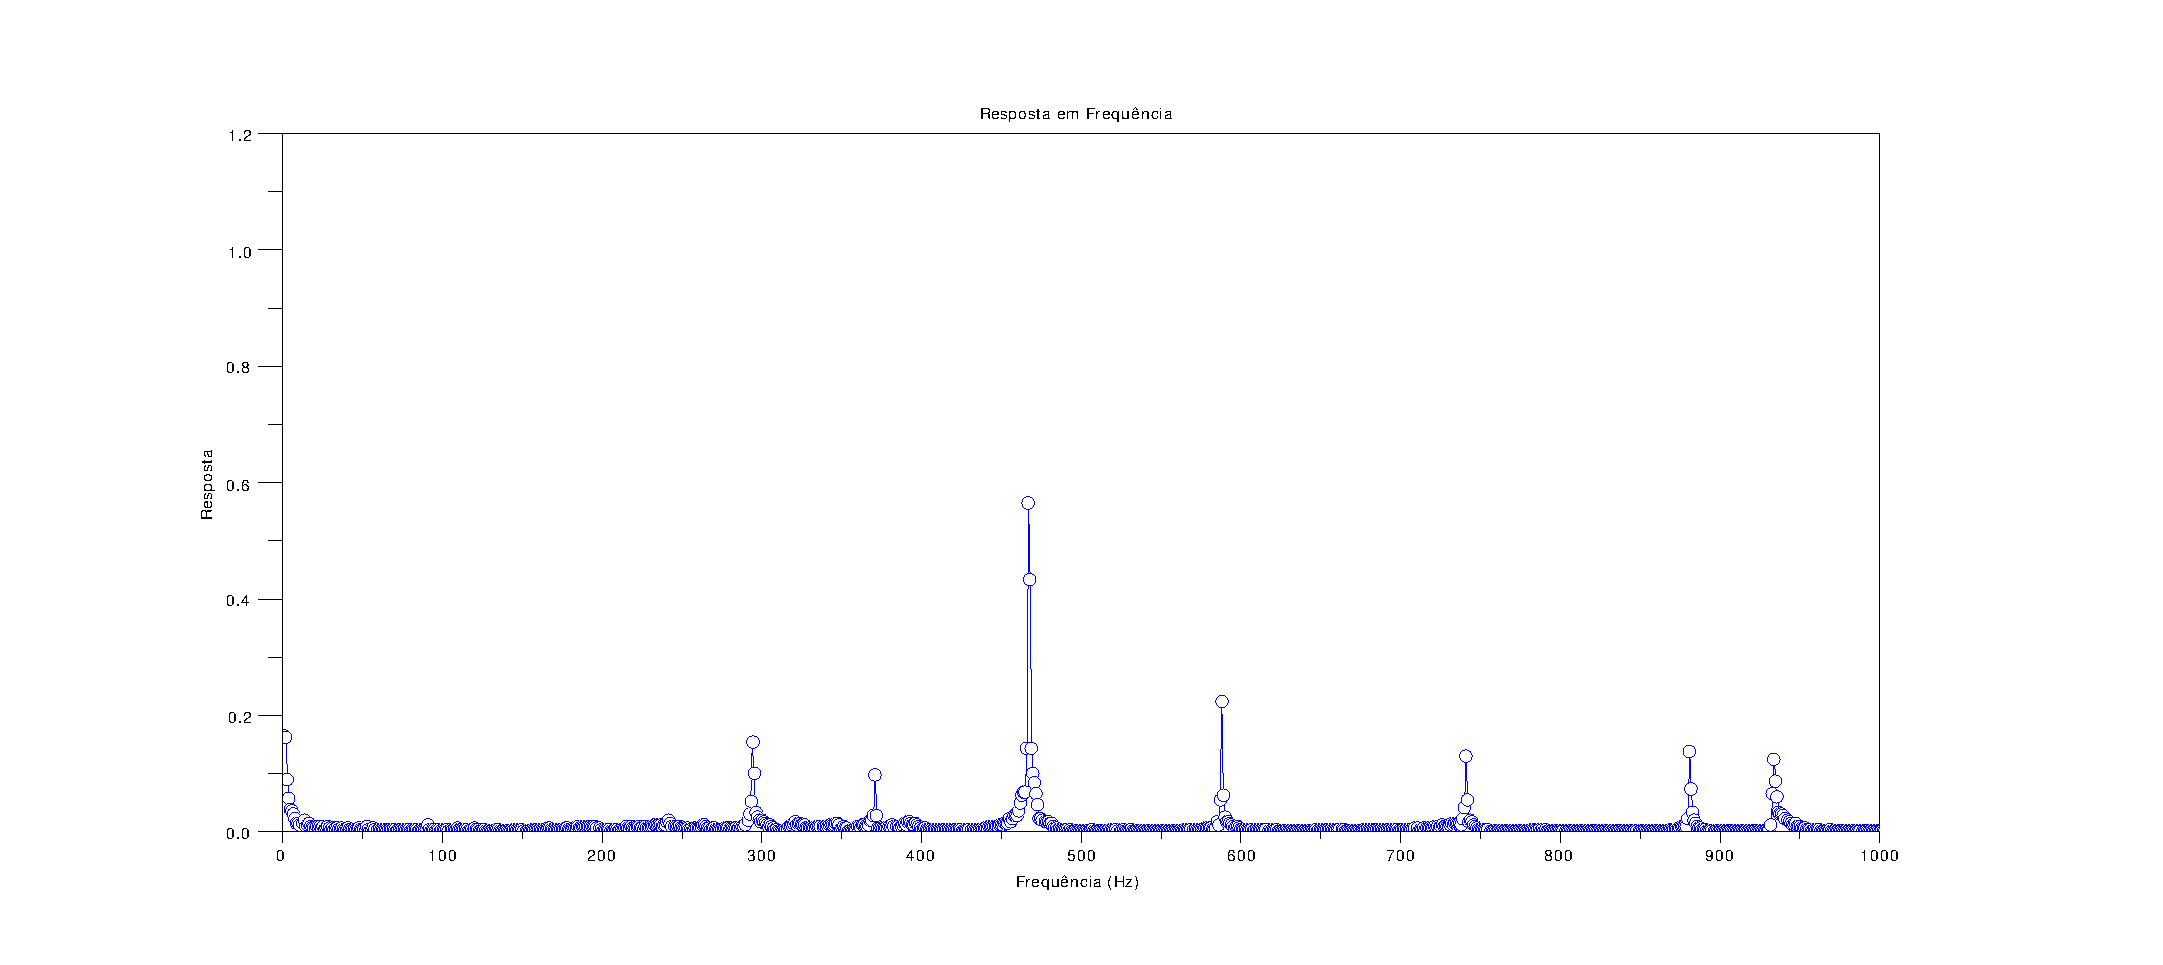
\includegraphics[keepaspectratio=true,scale=0.49]{figuras/Dm/fft_Daum.eps}
	\caption{Gráfico da resposta em frequência para a gravação do acorde $Daum$}
\end{figure}

\begin{figure}[h]
	\centering
		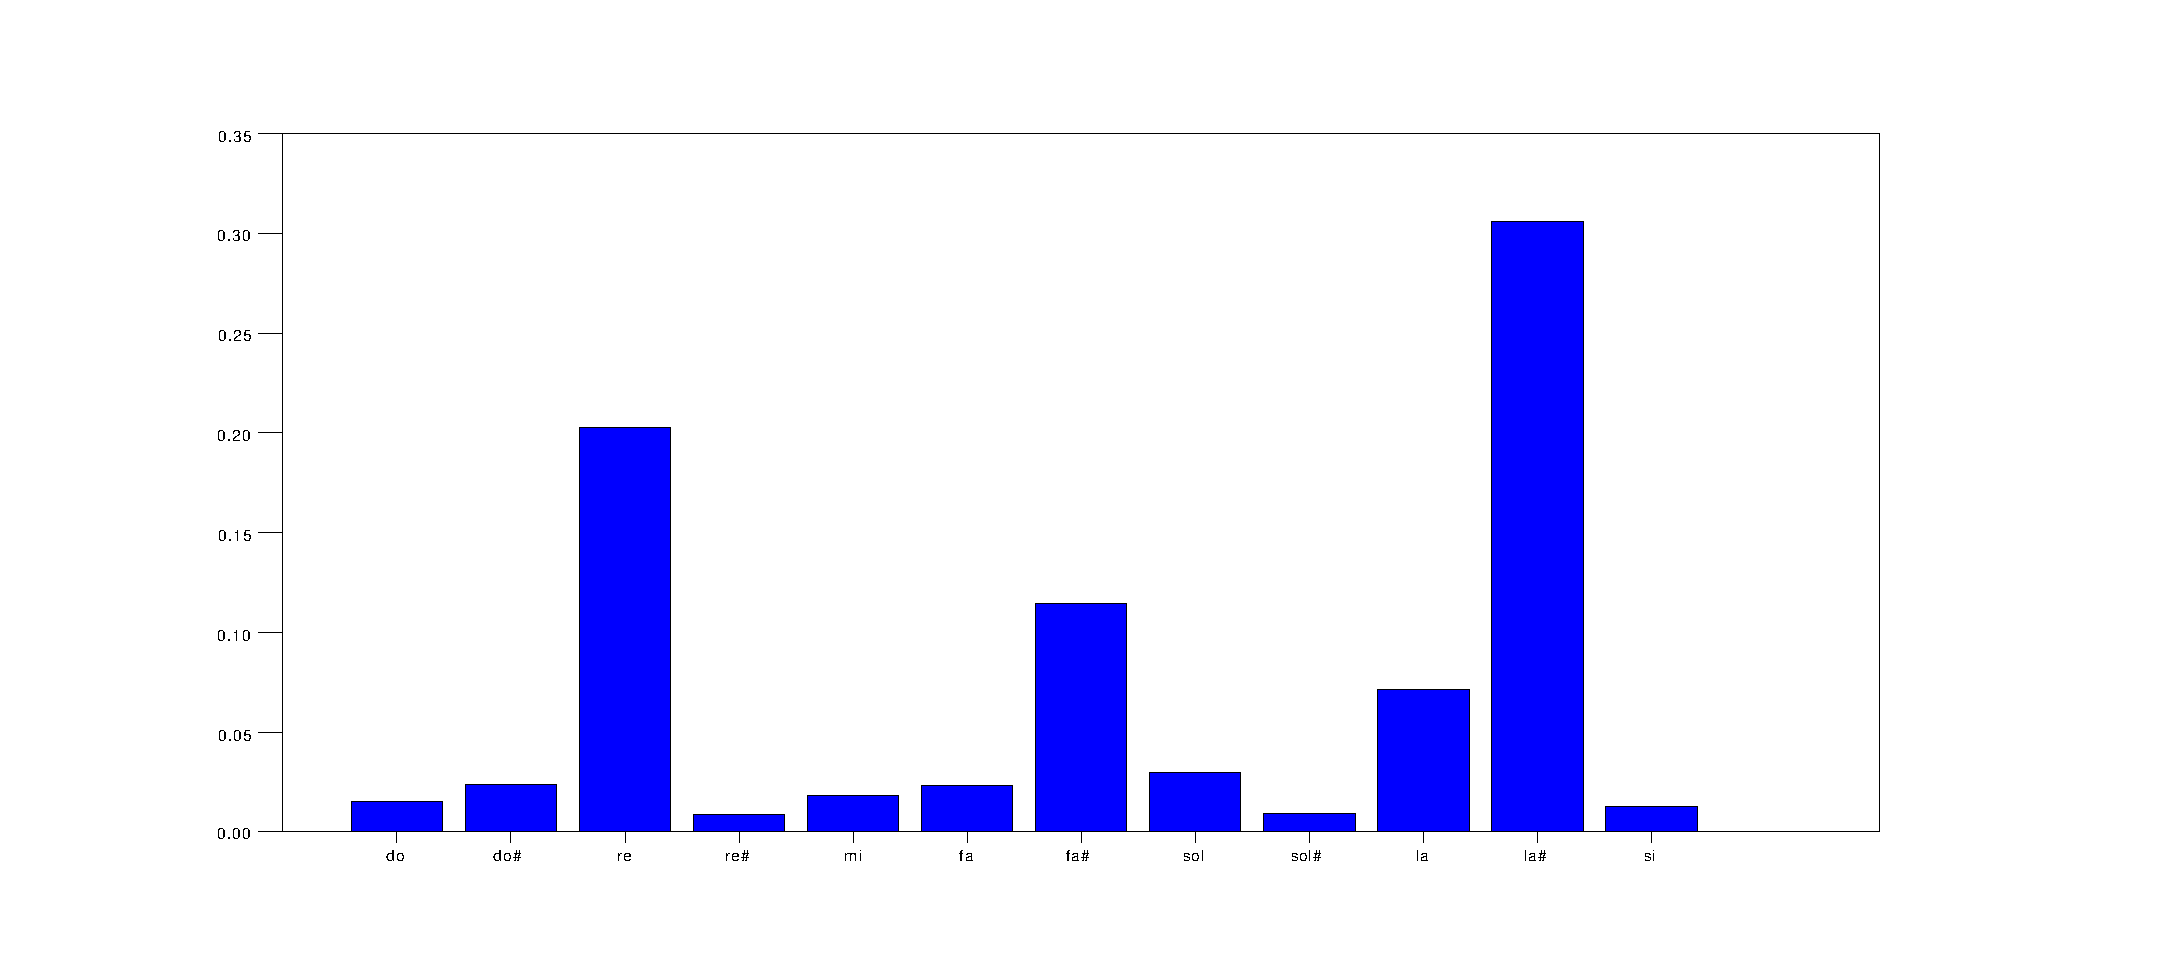
\includegraphics[keepaspectratio=true,scale=0.49]{figuras/Dm/notas_Daum.eps}
	\caption{Gráfico de sugestão de notas para a gravação do acorde $Daum$}
\end{figure}

\begin{figure}[h]
	\centering
		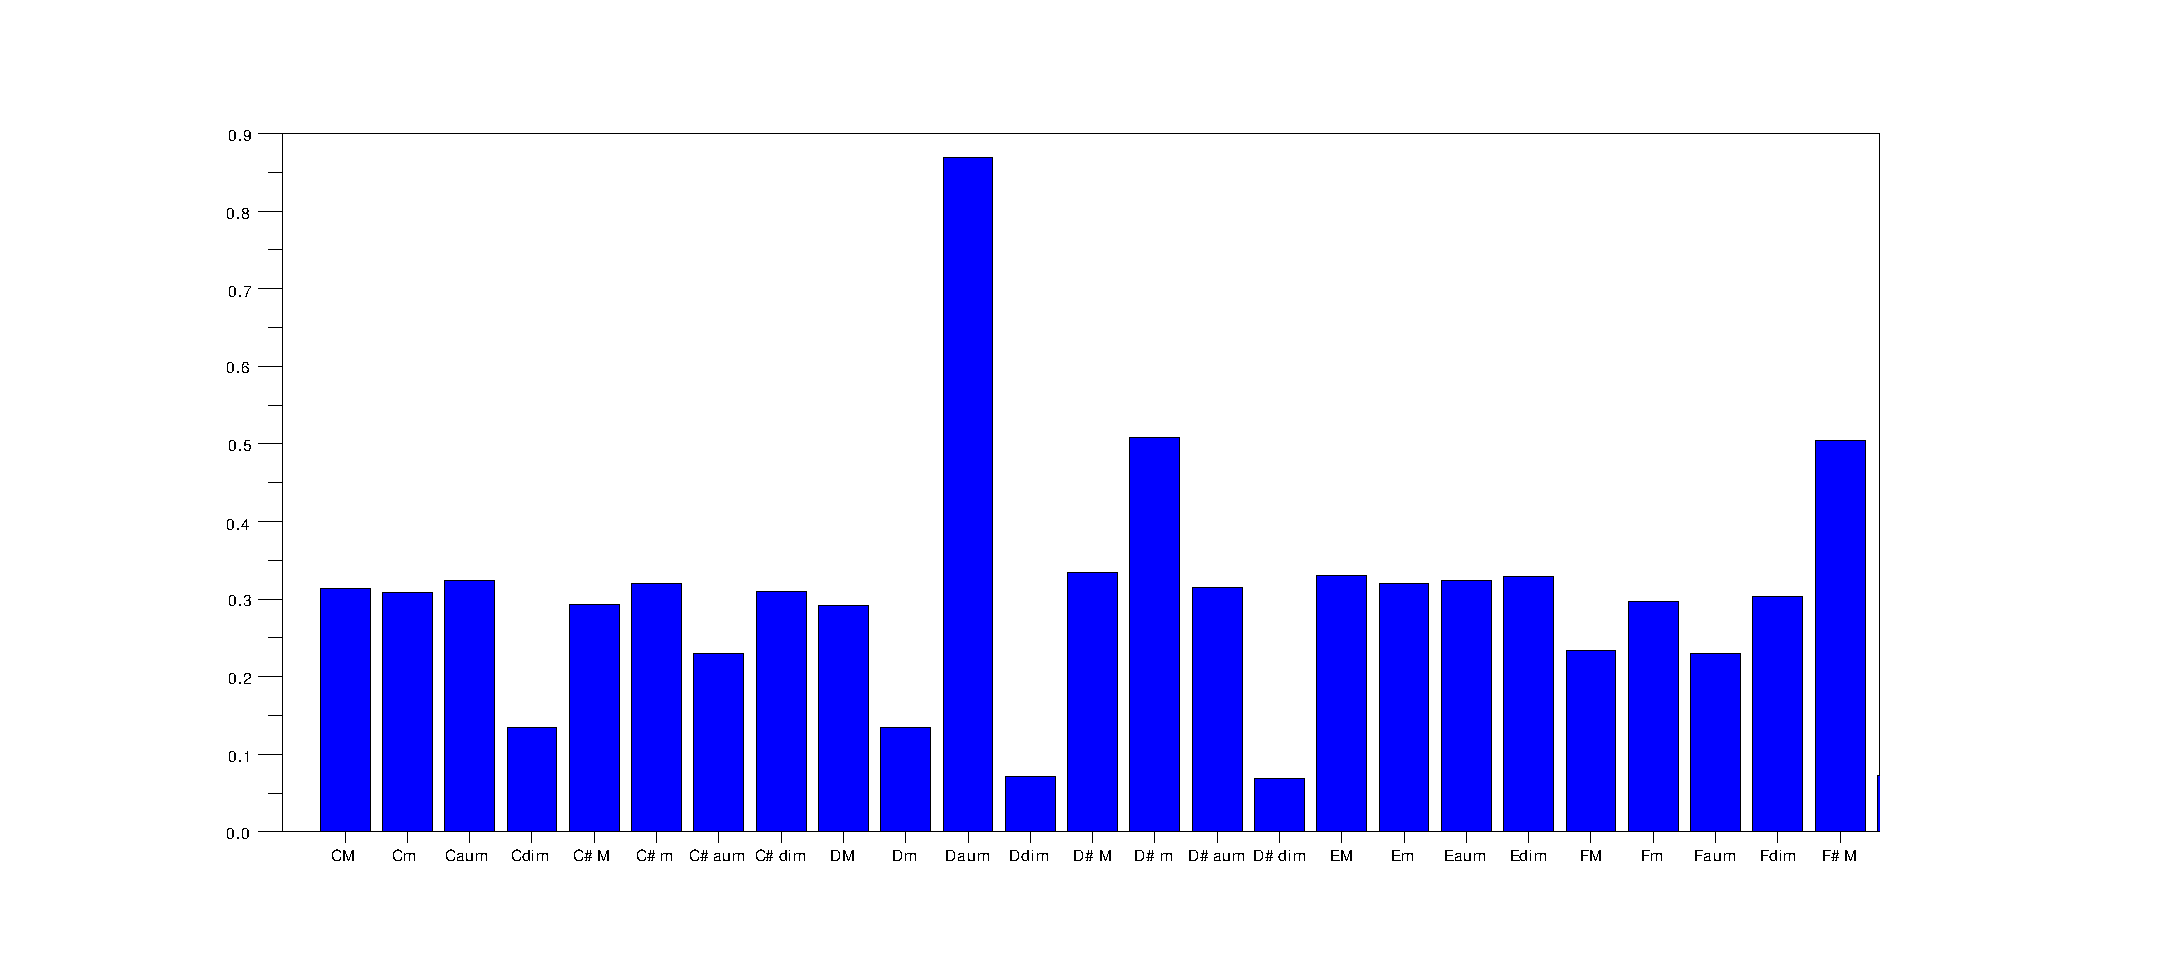
\includegraphics[keepaspectratio=true,scale=0.49]{figuras/Dm/acordes_1_Daum.eps}
		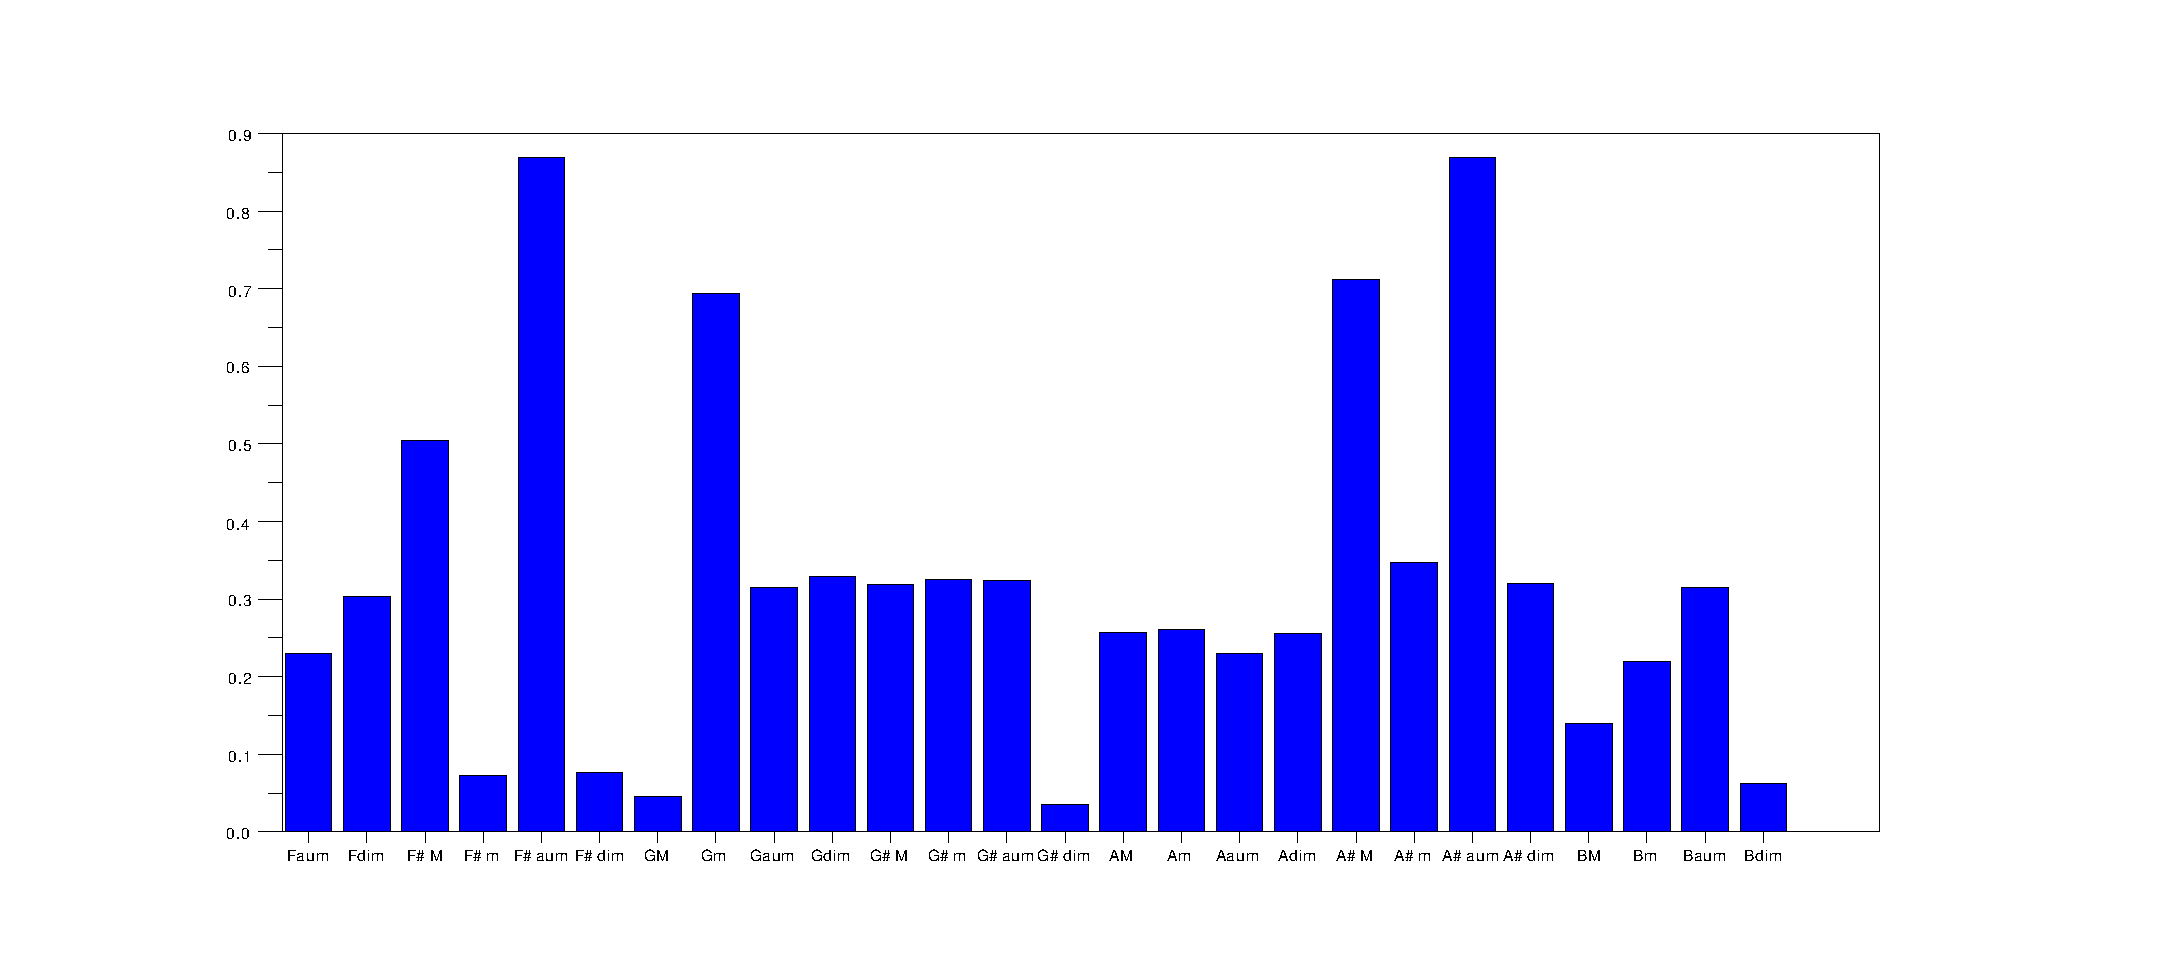
\includegraphics[keepaspectratio=true,scale=0.49]{figuras/Dm/acordes_2_Daum.eps}
	\caption{Gráficos de sugestão de acordes a gravação do acorde $Daum$}
\end{figure}
\newpage

Do resultado da primeira camada de processamento é gerado o gráfico da Figura 25. Esse gráfico diz respeito a natureza da composição do sinal em senoides em termos de transformada de fourier. O primeiro pico, no valor de 294 Hz, é relativo a nota $Ré$. O segundo pico, no valor de 371 Hz, é relativo a nota $Fá\#$. O terceiro pico, no valor de 467 Hz, é relativo a nota $Lá\#$. Os picos seguintes são relativos aos harmônicos dessas três notas.

Do resultado da segunda camada de processamento é gerado gráfico da Figura 26. É possível perceber nele que as notas $Ré$, $Fá\#$ e $Lá\#$ são as que mais possuem energia ou, no ponto de vista de sugestão, as mais sugeridas. De certa forma, essas mesmas notas compõe os acordes $F\#aum$ e $A\#aum$ causando um erro de redundância de informação no sistema.

Do resultado da terceira camada de processamento são gerados os gráficos da Figura 27. Essa camada é relativa ao resultados das sugestões de acordes musicais. É perceptível a alta sugestão dos acordes Daum, $F\#aum$ e $A\#aum$ com a mesma quantidade de energia. Isso é devido às notas comporem os mesmos acordes, diferenciando um do outro somente pela nota mais grave da tríade. Como o sistema não possui um módulo de detecção de baixos, esses 3 acordes são congruentes.



\section{Tabela de resultados dos acordes tocados}
\label{sec:tabelaacordestocados}
Segue a tabela de resultados do sistema dado um acorde tocado. Esses resultados foram gerados pelo script referenciado em anexo (Anexo, A11). Os acordes em negrito são aqueles que o sistema errou devido a falta de um módulo de software que diferenciasse as notas em termos de baixos e inversões, interpretando-as como tríades no modo fundamental. E esse fato é tão relevante que o sistema desconsidera as inversões.

Tais informações e mais outras estão referencidas na tabela a seguir:

\begin{table}[ht!]
%Vertical lines as column separators
 \centering
  \resizebox{0.9\textwidth}{!}{
\begin{tabular}{ | c | c | c | c |}
  \hline
  - & \textbf{Acorde Fundamental} & \textbf{Quinta Invertida} & \textbf{Terça Invertida}\\
  \hline
  \textbf{CM} & CM & CM & CM \\
  \hline
  \textbf{Cm} & Cm & Cm & Cm \\
  \hline
  \textbf{Caum} & Caum & Caum & Caum \\
  \hline
  \textbf{Cdim} & Cdim & Cdim & Cdim \\
  \hline
  \textbf{C\#M} & C\#M & C\#M & C\#M \\
  \hline
  \textbf{C\#m} & C\#m & C\#m & C\#m \\
  \hline
  \textbf{C\#aum} & C\#aum & C\#aum & C\#aum \\
  \hline
  \textbf{C\#dim} & C\#dim & C\#dim & C\#dim \\
  \hline
  \textbf{DM} & DM & DM & DM \\
  \hline
  \textbf{Dm} & Dm & Dm & Dm \\
  \hline
  \textbf{Daum} & Daum & Daum & Daum \\
  \hline
  \textbf{Ddim} & Ddim & Ddim & Ddim \\
  \hline
  \textbf{D\#M} & D\#M & D\#M & D\#M \\
  \hline
  \textbf{D\#m} & D\#m & D\#m & D\#m \\
  \hline
  \textbf{D\#aum} & D\#aum & D\#aum & D\#aum \\
  \hline
  \textbf{D\#dim} & D\#dim & D\#dim & D\#dim \\
  \hline
  \textbf{EM} & EM & EM & EM \\
  \hline
  \textbf{Em} & Em & Em & Em \\
  \hline
  \textbf{Eaum} & \textbf{Caum} & Caum & \textbf{Caum} \\
  \hline
  \textbf{Edim} & Edim & Edim & Edim \\
  \hline
  \textbf{FM} & FM & FM & FM \\
  \hline
  \textbf{Fm} & Fm & Fm & Fm \\
  \hline
  \textbf{Faum} & \textbf{C\#aum} & C\#aum & \textbf{C\#aum} \\
  \hline
  \textbf{Fdim} & Fdim & Fdim & Fdim \\
  \hline
  \textbf{F\#M} & F\#M & F\#M & F\#M \\
  \hline
  \textbf{F\#m} & F\#m & F\#m & F\#m \\
  \hline
  \textbf{F\#aum} & F\#aum & \textbf{F\#aum} & \textbf{F\#aum} \\
  \hline
  \textbf{F\#dim} & F\#dim & F\#dim & F\#dim \\
  \hline
  \textbf{GM} & GM & GM & GM \\
  \hline
  \textbf{Gm} & Gm & Gm & Gm \\
  \hline
  \textbf{Gaum} & \textbf{D\#aum} & D\#aum & \textbf{D\#aum} \\
  \hline
  \textbf{Gdim} & Gdim & Gdim & Gdim \\
  \hline
  \textbf{G\#M} & G\#M & G\#M & G\#M \\
  \hline
  \textbf{G\#m} & G\#m & G\#m & G\#m \\
  \hline
  \textbf{G\#aum} & \textbf{Caum} & \textbf{Caum} & Caum \\
  \hline
  \textbf{G\#dim} & G\#dim & G\#dim & G\#dim \\
  \hline
  \textbf{AM} & AM & AM & AM \\
  \hline
  \textbf{Am} & Am & Am & Am \\
  \hline
  \textbf{Aaum} & \textbf{C\#aum} & \textbf{C\#aum} & C\#aum \\
  \hline
  \textbf{Adim} & Adim & Adim & Adim \\
  \hline
  \textbf{A\#M} & A\#M & A\#M & A\#M \\
  \hline
  \textbf{A\#m} & A\#m & A\#m & A\#m \\
  \hline
  \textbf{A\#aum} & \textbf{F\#aum} & F\#aum & \textbf{F\#aum} \\
  \hline
  \textbf{A\#dim} & A\#dim & A\#dim & A\#dim \\
  \hline
  \textbf{BM} & BM & BM & BM \\
  \hline
  \textbf{Bm} & Bm & Bm & Bm \\
  \hline
  \textbf{Baum} & \textbf{D\#aum} & \textbf{D\#aum} & D\#aum \\
  \hline
  \textbf{Bdim} & Bdim & Bdim & Bdim \\
  \hline
\end{tabular}
}
\caption{Tabela de resultados dado os acordes tocados}
\label{tab:label_test}
\end{table}

\begin{table}[ht!]
  %Vertical lines as column separators
  \centering
  \resizebox{0.9\textwidth}{!}{
  \begin{tabular}{ | c | c | c | c |}
    \hline
    - & \textbf{Acorde Fundamental} & \textbf{Quinta Invertida} & \textbf{Terça Invertida}\\
    \hline
    \textbf{C} & C & C/G & C/E \\
    \hline
    \textbf{Cm} & Cm & Cm/G & Cm/D\# \\
    \hline
    \textbf{Caum} & Caum & G\#aum & Eaum \\
    \hline
    \textbf{Cdim} & Cdim & Cdim/F\# & Cdim/D\# \\
    \hline
    \textbf{C\#} & C\# & C\#/G\# & C\#/F \\
    \hline
    \textbf{C\#m} & C\#m & C\#m/G\# & C\#m/E \\
    \hline
    \textbf{C\#aum} & C\#aum & Aaum & Faum \\
    \hline
    \textbf{C\#dim} & C\#dim & C\#dim/G & C\#dim/E \\
    \hline
    \textbf{D} & D & D/A & D/F\# \\
    \hline
    \textbf{Dm} & Dm & Dm/A & Dm/F \\
    \hline
    \textbf{Daum} & Daum & A\#aum & F\#aum \\
    \hline
    \textbf{Ddim} & Ddim & Ddim/G\# & Ddim/F \\
    \hline
    \textbf{D\#} & D\# & D\#/A\# & D\#/G \\
    \hline
    \textbf{D\#m} & D\#m & D\#m/A\# & D\#m/F\# \\
    \hline
    \textbf{D\#aum} & D\#aum & Baum & Gaum \\
    \hline
    \textbf{D\#dim} & D\#dim & D\#dim/A & D\#dim/F\# \\
    \hline
    \textbf{E} & E & E/B & E/G\# \\
    \hline
    \textbf{Em} & Em & Em/B & Em/G \\
    \hline
    \textbf{Eaum} & Eaum & Caum & G\#aum \\
    \hline
    \textbf{Edim} & Edim & Edim/A\# & Edim/G \\
    \hline
    \textbf{FM} & F & F/C & F/A \\
    \hline
    \textbf{Fm} & Fm & Fm/C & Fm/G\# \\
    \hline
    \textbf{Faum} & Faum & C\#aum & Aaum \\
    \hline
    \textbf{Fdim} & Fdim & Fdim/B & Fdim/G\# \\
    \hline
    \textbf{F\#} & F\# & F\#/C\# & F\#/A\# \\
    \hline
    \textbf{F\#m} & F\#m & F\#m/C\# & F\#m/A \\
    \hline
    \textbf{F\#aum} & F\#aum & Daum & A\#aum \\
    \hline
    \textbf{F\#dim} & F\#dim & F\#dim/C & F\#dim/A \\
    \hline
    \textbf{G} & G & G/D & G/B \\
    \hline
    \textbf{Gm} & Gm & Gm/D & Gm/A\# \\
    \hline
    \textbf{Gaum} & Gaum & D\#aum & Baum \\
    \hline
    \textbf{Gdim} & Gdim & Gdim/C\# & Gdim/A\# \\
    \hline
    \textbf{G\#} & G\# & G\#/D\# & G\#/C \\
    \hline
    \textbf{G\#m} & G\#m & G\#m/D\# & G\#m/B \\
    \hline
    \textbf{G\#aum} & G\#aum & Eaum & Caum \\
    \hline
    \textbf{G\#dim} & G\#dim & G\#dim/D & G\#dim/B \\
    \hline
    \textbf{A} & A & A/E & A/C\# \\
    \hline
    \textbf{Am} & Am & Am/E & Am/C \\
    \hline
    \textbf{Aaum} & Aaum & Faum & C\#aum \\
    \hline
    \textbf{Adim} & Adim & Adim/D\# & Adim/C \\
    \hline
    \textbf{A\#} & A\# & A\#/F & A\#/D \\
    \hline
    \textbf{A\#m} & A\#m & A\#m/F & A\#m/C\# \\
    \hline
    \textbf{A\#aum} & A\#aum & F\#aum & Daum \\
    \hline
    \textbf{A\#dim} & A\#dim & A\#dim/E & A\#dim/C\# \\
    \hline
    \textbf{B} & B & B/F\# & B/D\# \\
    \hline
    \textbf{Bm} & Bm & Bm/F\# & Bm/D \\
    \hline
    \textbf{Baum} & Baum & Gaum & D\#aum \\
    \hline
    \textbf{Bdim} & Bdim & Bdim/F & Bdim/D \\
    \hline
  \end{tabular}
  }
  \caption{Tabela de resultados dado os acordes tocados com inversões}
  \label{tab:label_test}
\end{table}
